\documentclass[11pt,a4paper]{article}
\usepackage[margin=2.2cm]{geometry}
\usepackage{amsmath,amssymb}
\usepackage{graphicx}
\usepackage{booktabs}
\usepackage{tabularx}
\usepackage{xcolor}
\usepackage{enumitem}
\usepackage[hidelinks]{hyperref}
\usepackage{caption}
\captionsetup{font=small,labelfont=bf}
\setlist{itemsep=2pt,topsep=3pt}
\newcommand{\la}{\ell_a}
\newcommand{\status}[1]{\textbf{\textcolor{black!70}{[#1]}}}

\title{Overcharged Cavities: Project Status Report}
\author{Active nematic MPCD in cavities with imposed wall winding\\[2pt]
\small Prepared for Benjamin Loewe (with Claude), \today}
\date{}

\begin{document}
\maketitle
\tableofcontents
\bigskip

%=====================================================================
\section{Summary}
\textbf{Question.} An active nematic (NIAMH-MPCD) in a cavity whose homeotropic wall anchoring winds $k$ times
around the wall carries total topological charge $k$. In circles, the charge splits into a bulk of net
charge $+1$ (the Euler characteristic of the disc, as for planar anchoring) and a wall layer of charge $k-1$.
\emph{Is this split topological (set by $k$ and the topology of the cavity) or geometric (set by its shape)?}

\textbf{Main findings so far.}
\begin{itemize}
  \item \textbf{Circles} at the working activity $\zeta=0.07$: bulk $+1$, wall layer of $2k-2$ pinned $+\tfrac12$
        defects, for $k=2\dots10$ at $R/\la=1.43$ (3 seeds), and up to $R/\la\approx 2.2$. At $R/\la\approx 2.9$ the
        layer thickens and partly slides; the bulk value degrades to $\approx 1.8$--$1.9$.
  \item \textbf{Best observable:} the accumulated charge $Q(c)$ inside a level $c$ (circle: $c=r$). Circles show a
        plateau at $+1$ just inside the wall. Three independent edge criteria (pinned sites, mobility, orientation)
        agree on circles.
  \item \textbf{Activity (H3):} activity does not enter only through $\la$. Onset effects at $\zeta=0.05$ (unstable layer),
        compressibility at $\zeta\ge0.09$ (the vortex empties the cavity centre), closing layer--bulk gap at $0.11$.
        $\zeta=0.07$ balances both and is the working activity.
  \item \textbf{Ovals (H1, Cassini cavities, new code):} elongated cavities ($b/a=1.6\to1.02$, half-length $2.2$--$2.9\,\la$)
        show \emph{no} layer + bulk structure: $Q(c)$ rises smoothly with no plateau, wall defects leave the wall within
        $\sim$100--200 time units, while circles of the same size keep the layer.
        \textbf{Size control passed:} at half-length $1.53\,\la$ (where circles are cleanest) the layer depth $d^*/\la$ goes
        0.23, 0.30, 0.41, 0.50 for $b/a=2.5, 2.0, 1.6, 1.3$ against 0.20 for circles. There is a sharp crossover with the
        aspect ratio: 1.17 circle-like, 1.29 partial, $\gtrsim1.4$ lost, already for convex shapes.
        \textbf{The charge split is geometric.} The area fraction outside the $Q=+1$ level collapses onto one curve
        against the aspect ratio for ovals of all sizes (crossing $\frac12$ near aspect 1.5), while circles stay at 0.20--0.32.
  \item \textbf{Pinch-off:} as the neck closes the lobes do \emph{not} become independent cavities with their own $+1$;
        a single oval with one lobe's shape loses the layer too, so the lobe shape is what matters.
  \item \textbf{Weekend (Sec.~\ref{sec:weekend}):} circles keep the layer from 0.75 to $\approx2\,\la$ at all densities, and
        the ovals lose it inside that region (shape, not size); \textbf{ellipses lose it too} (aspect $\gtrsim1.5$); the area
        fraction collapses on aspect ratio with seeds; \textbf{mirror runs}: the bulk stays positive and reaches $+1$ only for
        $|k|\gtrsim13$ (activity breaks the mirror symmetry); a crowded wall (high $k$) restores the topological structure.
  \item \textbf{High winding} partly restores the layer in the pinched oval ($k=15$--20): the bulk returns towards $+1$
        for the whole cavity ($\approx+\frac12$ per lobe), i.e.\ a crowded wall favours the topological picture.
\end{itemize}

\textbf{Decisions.} Working activity $\zeta=0.07$; present density stratification as part of the MPCD result.
If the geometric effect is confirmed, the ovals go into paper~1 (to be discussed with Tyler); future server runs
will be ovals; ellipses become an office-machine exploration (``can a convex cavity lose the layer?'').

%=====================================================================
\section{Model, cavities and anchoring}
\begin{itemize}
  \item \textbf{Solver:} NIAMH-MPCD (Shendruk Lab), 2D, collision operator 21 (density-modulated active dipole),
        nematic LC on (\texttt{lc} 1), mean density 20 particles per cell, $k_BT=1$, $\Delta t=0.1$.
  \item \textbf{Cavities:} no-slip walls with phantom particles, homeotropic anchoring
        (\texttt{MUN} 1, \texttt{MUT} 0).
        \emph{Circles} of radius $R$. \emph{Cassini ovals} $d_1 d_2 = b^2$ with foci at $(\pm a,0)$: convex for
        $b/a\ge\sqrt2$, concave neck for $1<b/a<\sqrt2$, lemniscate at $b=a$; half-length $\sqrt{a^2+b^2}$,
        waist $2\sqrt{b^2-a^2}$.
  \item \textbf{Custom anchoring} (\texttt{customAnch} $k$): the anchoring axis turns $k$ times around the wall.
        \texttt{eMode} selects how the winding is distributed: 0 normal angle (circles), 1 ellipse parameter,
        2 arclength (ellipses; validated), 3 arclength labelled by the polar angle (Cassini, needed because the
        normal angle runs backwards on a concave neck).
  \item \textbf{Resolution limit:} the imposed defect spacing $P/2k$ must stay $\gtrsim 6.7$ cells
        (density $2k/P\le0.15$; Table~\ref{tab:res}). This also limits $k$ in a given oval (e.g.\ $k\le18$ for the
        half-length-48 oval with $b/a=1.02$, perimeter 240).
\end{itemize}

\begin{table}[h]\centering\small
\caption{Resolution limit of the custom anchoring (passive and active alike; depends only on the spacing).}\label{tab:res}
\begin{tabular}{cccl}\toprule
$\rho=2k/P$ & spacing (cells) & frames passing the charge audit & verdict\\\midrule
0.10 & 10  & 99--100\% & clean\\
0.15 & 6.7 & 92--100\% & good\\
0.20 & 5.0 & 78--93\%  & degraded\\
$\ge0.25$ & $\le4$ & $\le30\%$ & fails\\\bottomrule
\end{tabular}
\end{table}

%=====================================================================
\section{Code and data infrastructure}
\subsection{Bugs found and fixed}
{\sloppy\begin{itemize}
  \item \textbf{Input seed ignored} (all NIAMH-MPCD users with a fixed seed): the RNG self-seeded from time+pid before the
        input seed was applied, while the synopsis reported the input seed. Fixed in the office build (29 Sep).
        All runs before the fix (including server batches 1--3) have effectively random seeds: statistically
        independent and valid, but not bit-reproducible. The server binary will be rebuilt after the sweeps.
  \item \textbf{Defect tracker:} legacy clustering could split U-shaped clusters, skipped the outer cell layer and did
        not wrap periodic boundaries (in PBC boxes only 64\% of frames charge-neutral). New union-find tracker
        (98\%); identical to the legacy tracker in cavities (251/251 frames). Legacy kept as an option.
  \item \textbf{Checkpoints did not store \texttt{customAnch}/\texttt{eMode}} (a restart would lose the anchoring);
        domain walls created by \texttt{domainWalls} had them uninitialised. Fixed on the \texttt{cassini} branch.
  \item Open: checkpoint restarts segfault (also in the production build); the Makefile header-dependency fix
        exists only in the upstream patch set; rotated ellipses (\texttt{O[2]}) need care.
\end{itemize}\par}
\subsection{Code, repository, reports}
\begin{itemize}
  \item Production tree \texttt{mpcd/} = upstream 2a38960 (PR \#160) + seed fix + tracker + custom anchoring
        (eMode 0/1/2). Private GitHub \texttt{baloewey/NIAMH-MPCD-overcharged}: \texttt{main} = production;
        branch \texttt{cassini} adds the checkpoint fix and Cassini walls + eMode 3 (validated, Section~\ref{sec:ovals}).
  \item Upstream bug report and patches ready (\texttt{reports/upstream\_patches/}, rebased on upstream a2cf7b2); not sent.
  \item Pages: collaborator brief (v4), defect-geography report, bug report (private web pages).
\end{itemize}
\subsection{Analysis tools (all in \texttt{runs/cavity/} and \texttt{runs/cassini/})}
{\sloppy
Charge audit; site rule (\texttt{edge\_sites.py}); spatial maps, profiles, ring-resolved $g(r\,|\,s)$
(\texttt{defect\_spatial.py}); mobility/orientation criteria (\texttt{edge\_criteria.py}); gap-closing tracker
(\texttt{defect\_tracks.py}, link radius 8, gap 4, 89--96\% of track starts/ends paired as $\pm\frac12$ events);
wall-defect label tracking (\texttt{bc\_labels.py}); Cassini tools (\texttt{gen\_cassini.py}, \texttt{cassini\_charge.py},
\texttt{lobe\_profiles.py}, \texttt{render\_cassini.py}, \texttt{fig\_accumulated\_charge.py}); Mathematica explorers
(\texttt{cassini\_oval\_manipulate.wl}).\par}

%=====================================================================
\section{Calibration: active length and compressibility}
$\la=\sqrt{A/\langle N\rangle}$ from the mean defect number in periodic boxes (transient removed, errors with time
correlations). Reference: $200^2$ box.
\begin{table}[h]\centering\small
\caption{Active length (cells). $200^2$ values at 0.06 and 0.11 are the mean of two seeds (seed spread 1.2--1.5$\sigma$).}
\begin{tabular}{lccccc}\toprule
$\zeta$ & 0.05 & 0.06 & 0.07 & 0.09 & 0.11\\\midrule
$\la$, $100^2$ box & $27.5\pm1.1$ & $22.9\pm0.4$ & $21.4\pm0.5$ & $20.2\pm0.4$ & --\\
$\la$, $200^2$ box & $26.2\pm0.2$ & $24.3\pm0.1$ & $\mathbf{22.2\pm0.3}$ & $20.7\pm0.1$ & $19.1\pm0.1$\\\bottomrule
\end{tabular}
\end{table}
No significant finite-size effect between the boxes. $\la\propto\zeta^{-1/2}$ up to $\zeta\approx0.08$, flattening above.
\textbf{Compressibility:} density SD $6.1\to9.8$ (Poisson 4.47) and rms Mach $0.66\to1.0$ from $\zeta=0.05$ to $0.09$
in boxes. In cavities, the vortex centrifuges particles to the wall (Table~\ref{tab:dens}).

\begin{table}[h]\centering\small
\caption{Occupancy in cavities ($k=8$, $R=1.43\,\la$): mean particles per cell by distance $s$ from the wall.}\label{tab:dens}
\begin{tabular}{lccccc}\toprule
$\zeta$ & spread / Poisson & $s<5$ & $s=10$--20 & centre $s>20$ & centre cells with $n<10$\\\midrule
0.07 & 1.5 & 25 & 17 & 14 & 15\%\\
0.09 & 2.0 & 28 & 14 & 9 & 60\%\\
0.11 & 2.2 & 29 & 13 & 8 & 70\%\\\bottomrule
\end{tabular}
\end{table}
Empty cells occur only at $\zeta\ge0.07$ ($\le8\times10^{-5}$ of interior cells), all near the vortex core. A low-Mach
control (higher $k_BT$) would change viscosity, nematic parameters and $\la$, i.e.\ the whole calibration:
\textbf{to discuss with Tyler.}

%=====================================================================
\section{Circular cavities}
\subsection{Validation}
Passive ($R=15$, $k=\pm1\dots\pm5$): wall director follows the imposed winding (alignment 0.96--0.99), exactly
$2|k|$ defects of the sign of $k$, net charge $k$ in 100\% of frames, bulk charge 0 for $|k|\ge2$ (all defects
in a 2--3 cell wall layer). Active reproduction ($k=5$, $R=15.9$): bulk $+1$ in 94\% of frames.
\subsection{Layer + bulk structure}
\begin{figure}[h]\centering
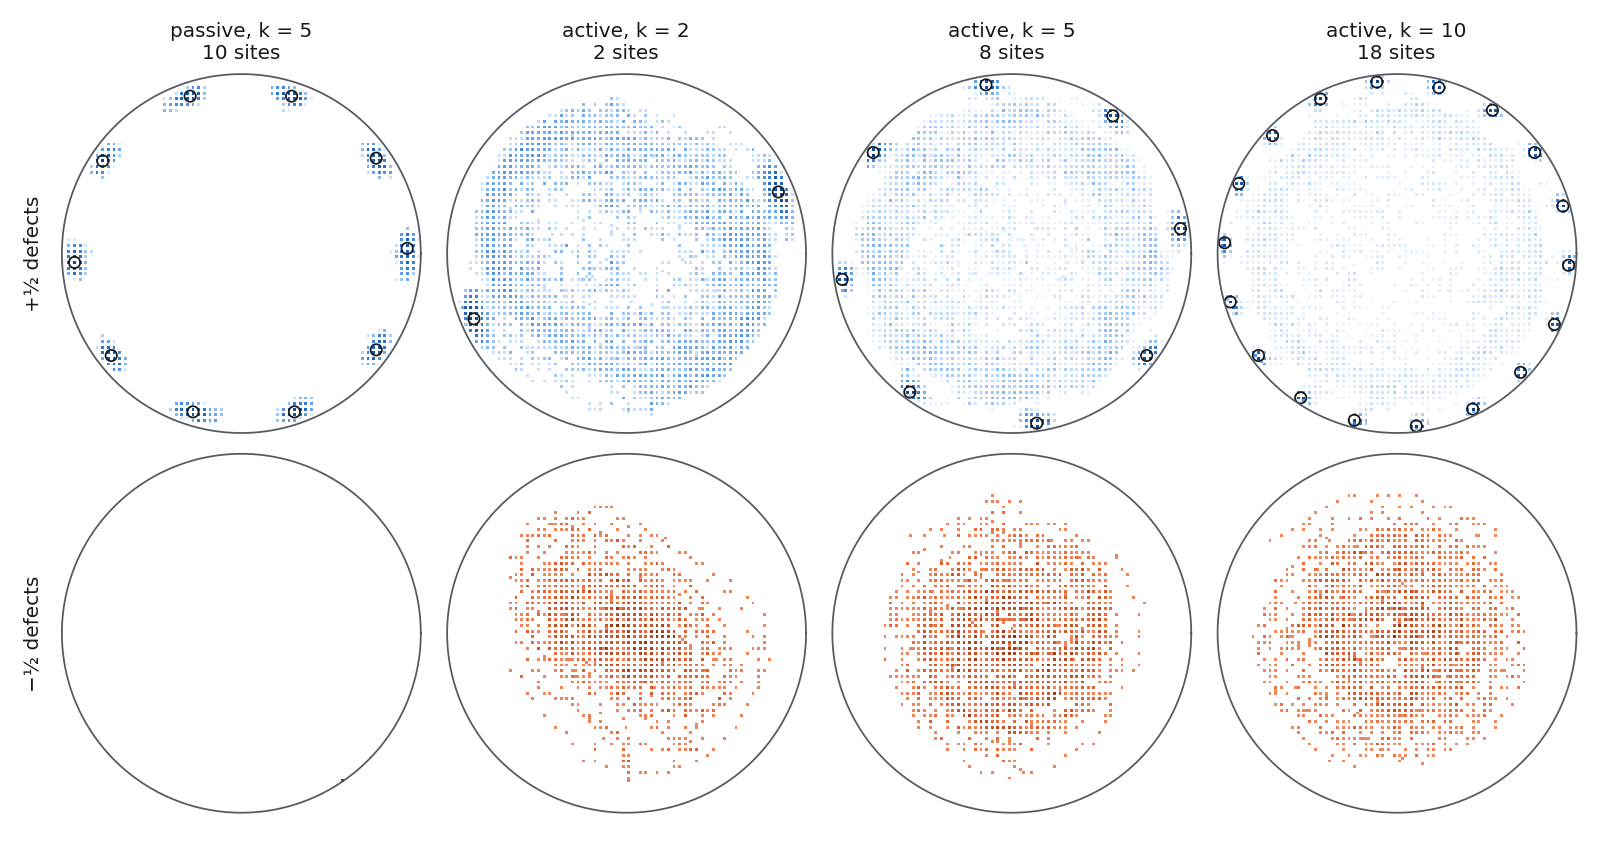
\includegraphics[width=\textwidth]{figs/circle_maps.png}
\caption{Time-averaged density of $+\frac12$ (top) and $-\frac12$ (bottom) defects. Passive $k=5$; active $k=2,5,10$
($\zeta=0.07$, $R=1.43\,\la$). Open circles: pinned sites ($2k$ passive, $2k-2$ active).}
\end{figure}
\begin{itemize}
  \item Wall $+\frac12$ sit on \textbf{fixed sites}: $2k-2$ in every active run (27/27), $2k$ passive.
  \item Radial profile: sharp $+\frac12$ peak at $s\approx1.2$ cells, a gap at $s\approx3$--4.5, a flat bulk; wall defects
        move at the tracker jitter floor (0.2--0.35 cells/time), bulk ones at 0.8--1.0.
  \item Bulk charge (site rule, 3 seeds, $R=1.43\,\la$): $\langle q_b\rangle=1.01$--$1.05$ for $k=2\dots9$,
        $P(q_b=+1)=0.89$--$0.96$.
  \item Wall defects are \textbf{tilted $\approx 63^\circ$ (1.03--1.13 rad) to the wall normal}, sign = vortex sense
        (6/6 runs), almost independent of $k$; bulk $+\frac12$ at $\approx2.4$ rad.
  \item Mobility and orientation criteria each agree with the site rule on 97--99\% of $+\frac12$ (Fig.~\ref{fig:crit}).
\end{itemize}
\begin{figure}[h]\centering
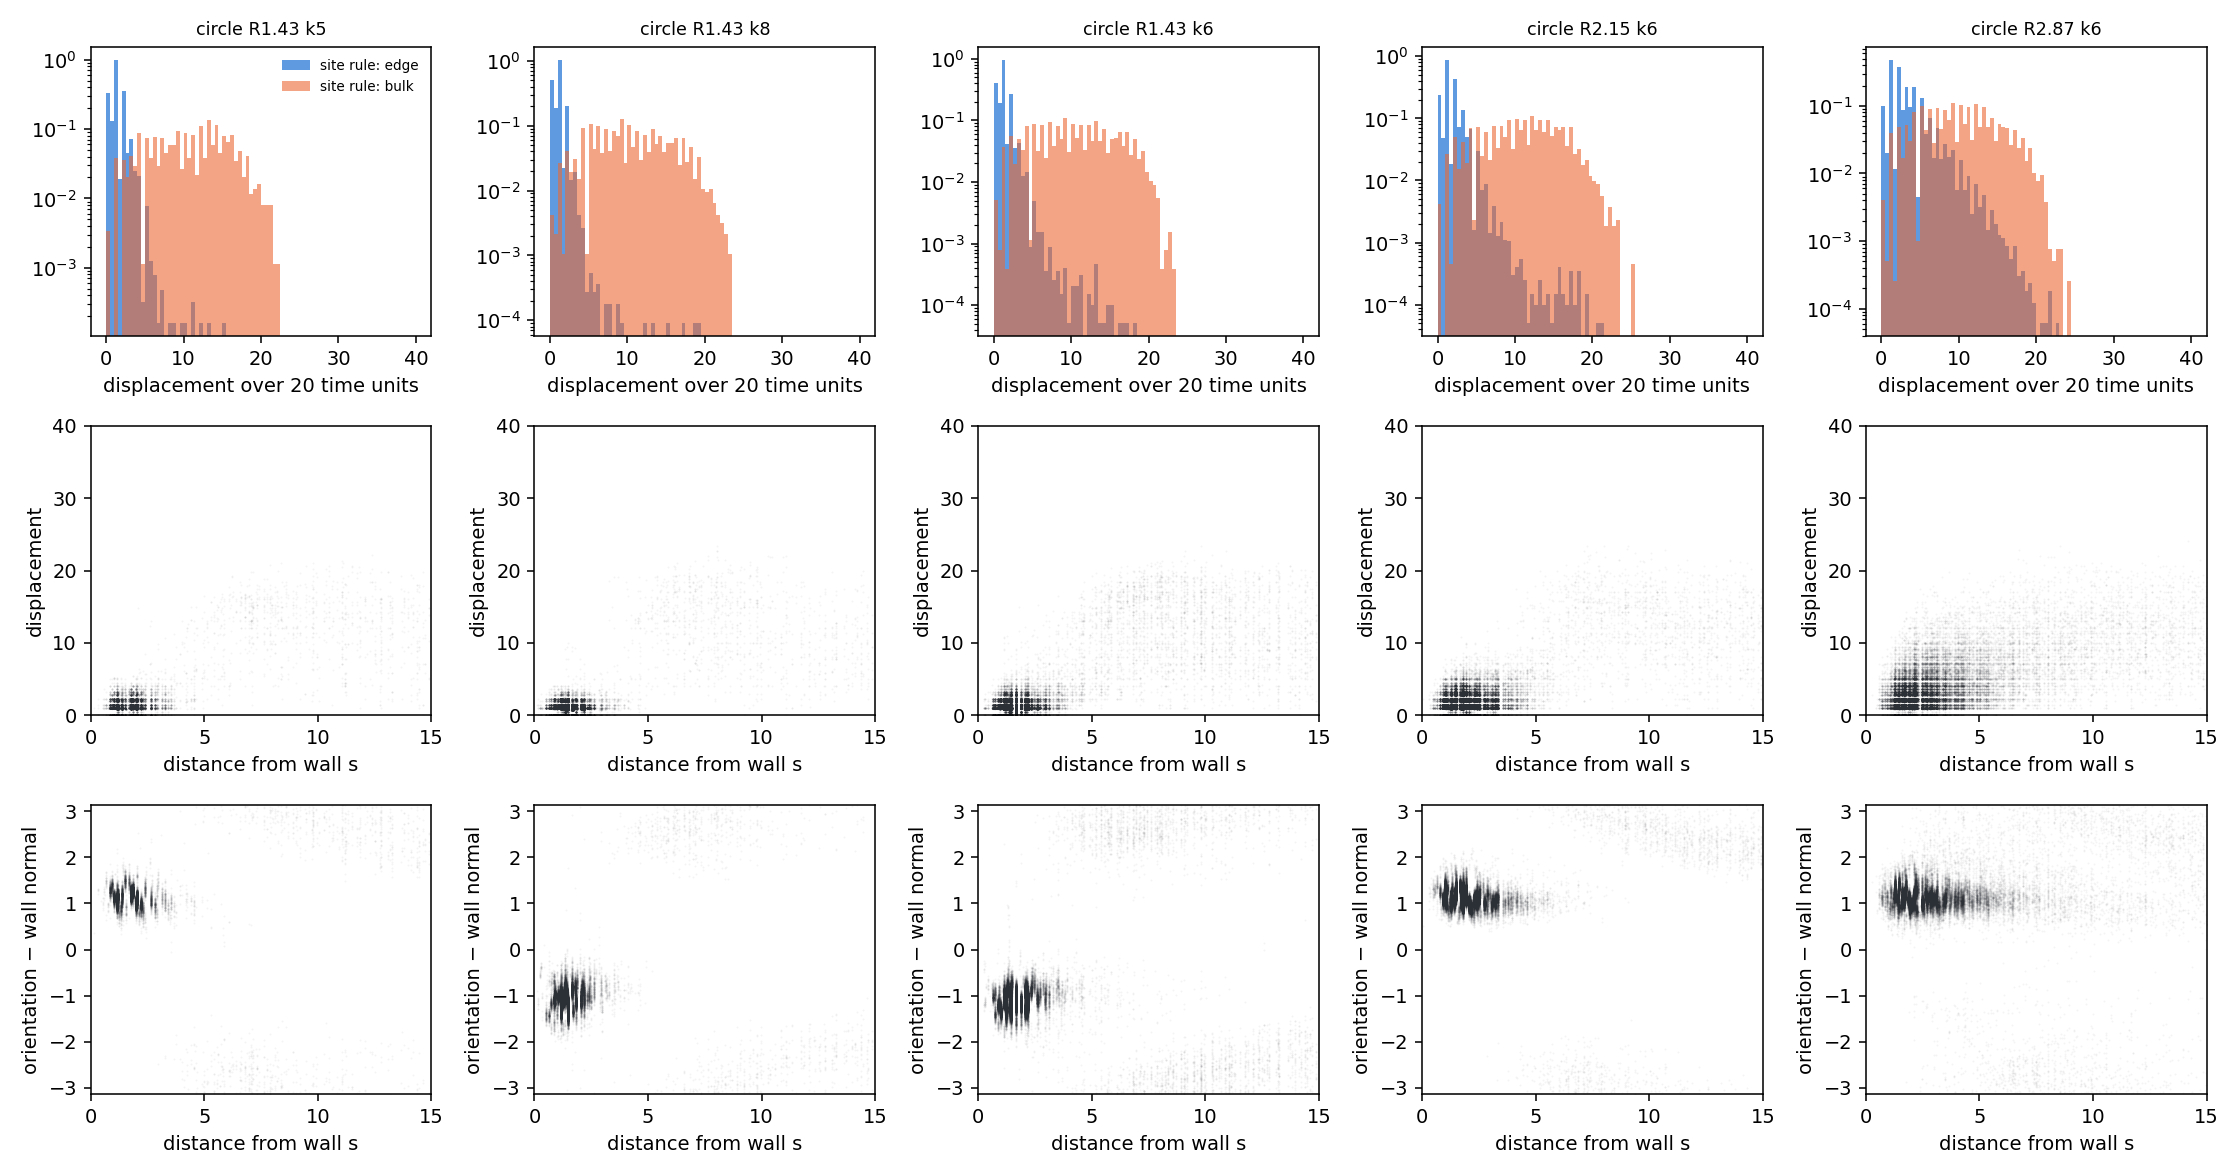
\includegraphics[width=\textwidth]{figs/edge_criteria_circles.png}
\caption{Cut-free criteria on circles. Top: displacement over 20 time units, split by the site rule. Middle/bottom:
displacement and orientation relative to the wall normal versus distance from the wall.}\label{fig:crit}
\end{figure}
\subsection{Pair correlations}
Ring-resolved $g(r\,|\,s)$ (reference defect binned by its ring, partner anywhere, radial profile divided out):
like charges have the same correlation hole ($g\approx0$ below $0.1R$, back to 1 by $0.5$--$0.6R\approx\la$);
opposite charges are bound at short range ($g\approx3.2$ at 2.5 cells). In $r/R$ ($\propto r/\la$) the $++$ curve
collapses for $\zeta=0.05$--$0.09$; $--$ only up to $\sim0.5R$ at $\zeta=0.05$.
\subsection{Size dependence ($k=6$, server sweep)}
Near-wall $+\frac12$ (within 3 cells; $2k-2=10$) and enclosed charge beyond $s=5$:
$R/\la=1.43$: 9.7, 0.99; $1.72$: 9.6, 0.99; $2.15$: 8.8, 1.06; $2.87$: 6.2, 1.80.
At $2.87\,\la$ the layer thickens and part of it slides (tilted but mobile). Wall-defect labels stay at the wall for
$\gg1000$ time units up to $2.15\,\la$ (84--94\% after 1000).

%=====================================================================
\section{Activity (H3)}
All at $R=1.434\,\la$, $k=2\dots10$, 3 seeds (0.09: seed 1 in the table; seeds 2--3 finished tonight).
\begin{table}[h]\centering\small
\caption{Activity scan at fixed $R/\la$. Gap depth: $+\frac12$ density at $s\approx3$--4.5 relative to the bulk. Plateau slope: d$Q$/d$s$ between $s=3$ and 5 ($k=8$).}
\begin{tabularx}{\textwidth}{lccccX}\toprule
$\zeta$ & $q_b$ & $P(q_b=+1)$ & gap & slope & failure mode\\\midrule
0.05 & 1.16--1.81 & 0.31--0.68 & -- & -- & onset: vacant sites, vortex reversals at $k=9,10$\\
0.06 & 1.05--1.15 & 0.67--0.83 & shallow & 0.13 & mild onset\\
\textbf{0.07} & \textbf{1.01--1.09} & \textbf{0.89--0.96} & $\sim5\times$ & \textbf{0.07} & clean\\
0.09 & 0.99--1.08 & 0.79--0.92 & $\sim4\times$ & 0.15 & centre depleted (compressibility)\\
0.11 & unclear ($k\ge7$) & 0.6--0.8 ($k\le6$) & $\sim1.5\times$ & 0.32 & gap closes; centre depleted\\\bottomrule
\end{tabularx}
\end{table}
\textbf{Conclusion:} activity does not enter only through $\la$; the clean regime is $\zeta\approx0.07$.
The layer has a fixed width in cells while the bulk density grows as $1/\la^2$, so the layer--bulk gap closes at
high activity.

%=====================================================================
\section{Ovals: Cassini cavities (H1, H8)}\label{sec:ovals}
\subsection{Implementation and validation}
New wall type on branch \texttt{cassini}: $W=d_1d_2-b^2$ (scales like the circle's $r^2-R^2$, identical for $a=0$),
normal $\nabla(d_1d_2)$, secant crossing times, eMode 3, setup guards, synopsis and checkpoint output.
Passive $k=3$: $a=0$ reproduces the circle (alignment 0.970/0.961 vs 0.971, accessible volume 706.8 vs 706.9);
$b/a=1.6$ and 1.2: alignment 0.976, audit 100\%. Tightest necks ($b/a=1.01$--1.02, waist $\approx13$ cells, $k=6$):
alignment 0.93, audit 100\%, all 12 imposed $+\frac12$ present.
\begin{figure}[h]\centering
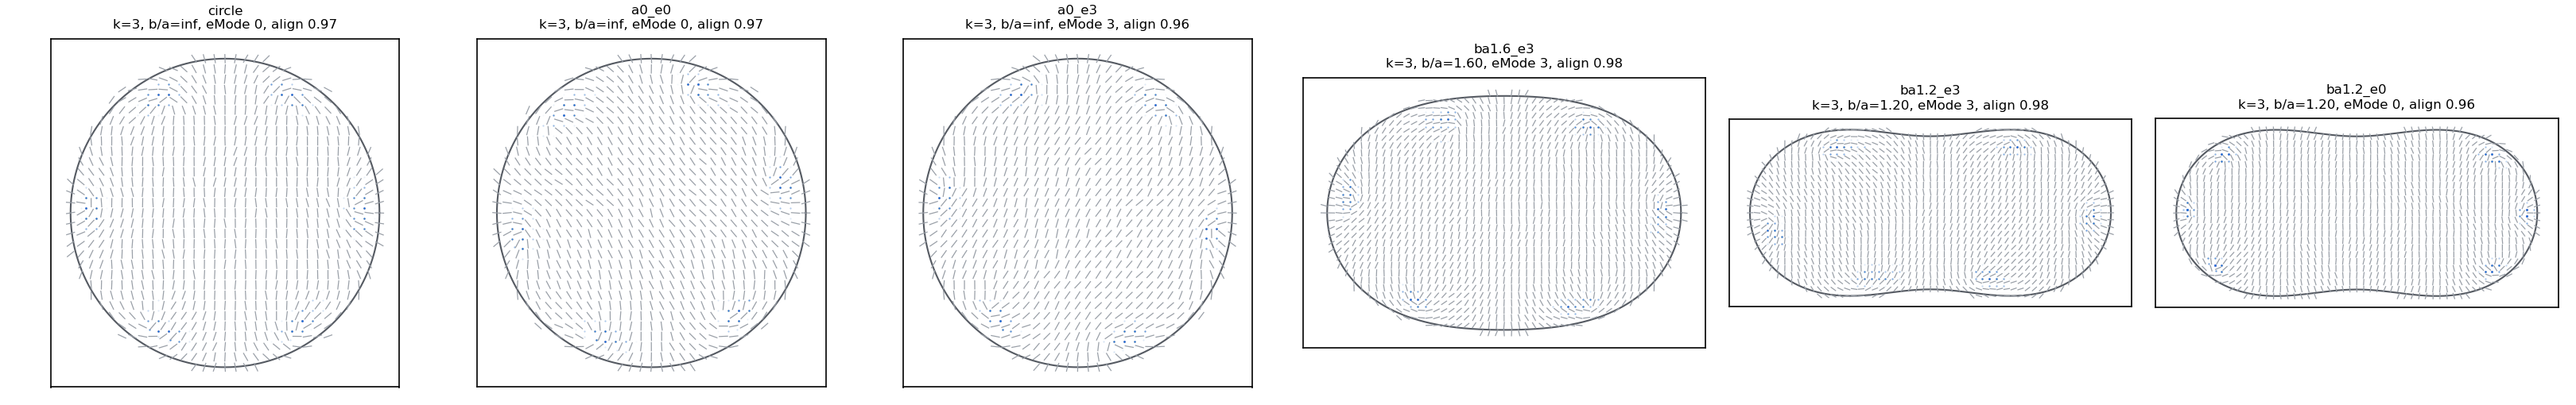
\includegraphics[width=\textwidth]{figs/cassini_validation.png}
\caption{Passive validation ($k=3$): circle reference, $a=0$ with eMode 0 and 3, and ovals $b/a=1.6$, 1.2 (eMode 3 and 0).}
\end{figure}
\subsection{Active ovals: what we see}
\begin{itemize}
  \item \textbf{Two vortices}, one per lobe, already at $b/a=1.6$ (convex); the rotation sense reverses over time;
        relative sense (co-/counter-rotating) not monotonic in neck width (1 seed each; tentative).
  \item \textbf{No wall layer:} the site rule finds only 3--7 sites; only $\sim$4--5.5 of the 12 imposed $+\frac12$
        behave like wall defects (slow and tilted); the defect density rises smoothly towards the wall with no gap.
  \item \textbf{Accumulated charge} (Fig.~\ref{fig:Qc}): circles show a $-\frac12$ core (negative $Q$), a plateau at $+1$ and a
        jump to $k$ at the wall; ovals rise smoothly, never negative, no plateau; all ovals fall on one curve.
  \item \textbf{Wall defects leave the wall} (Fig.~\ref{fig:labels}): in ovals only 6--39\% of labelled wall defects are
        at the wall after 1000 time units (circles 84--94\% up to $2.15\,\la$).
  \item Lobe coordinates: $w=z^2-a^2$ maps the Cassini levels to circles $|w|=c^2$ and their orthogonal hyperbolas to
        rays; focus-to-wall curves $z(c;\varphi)=\pm\sqrt{a^2+c^2e^{i\varphi}}$.
\end{itemize}
\begin{figure}[h]\centering
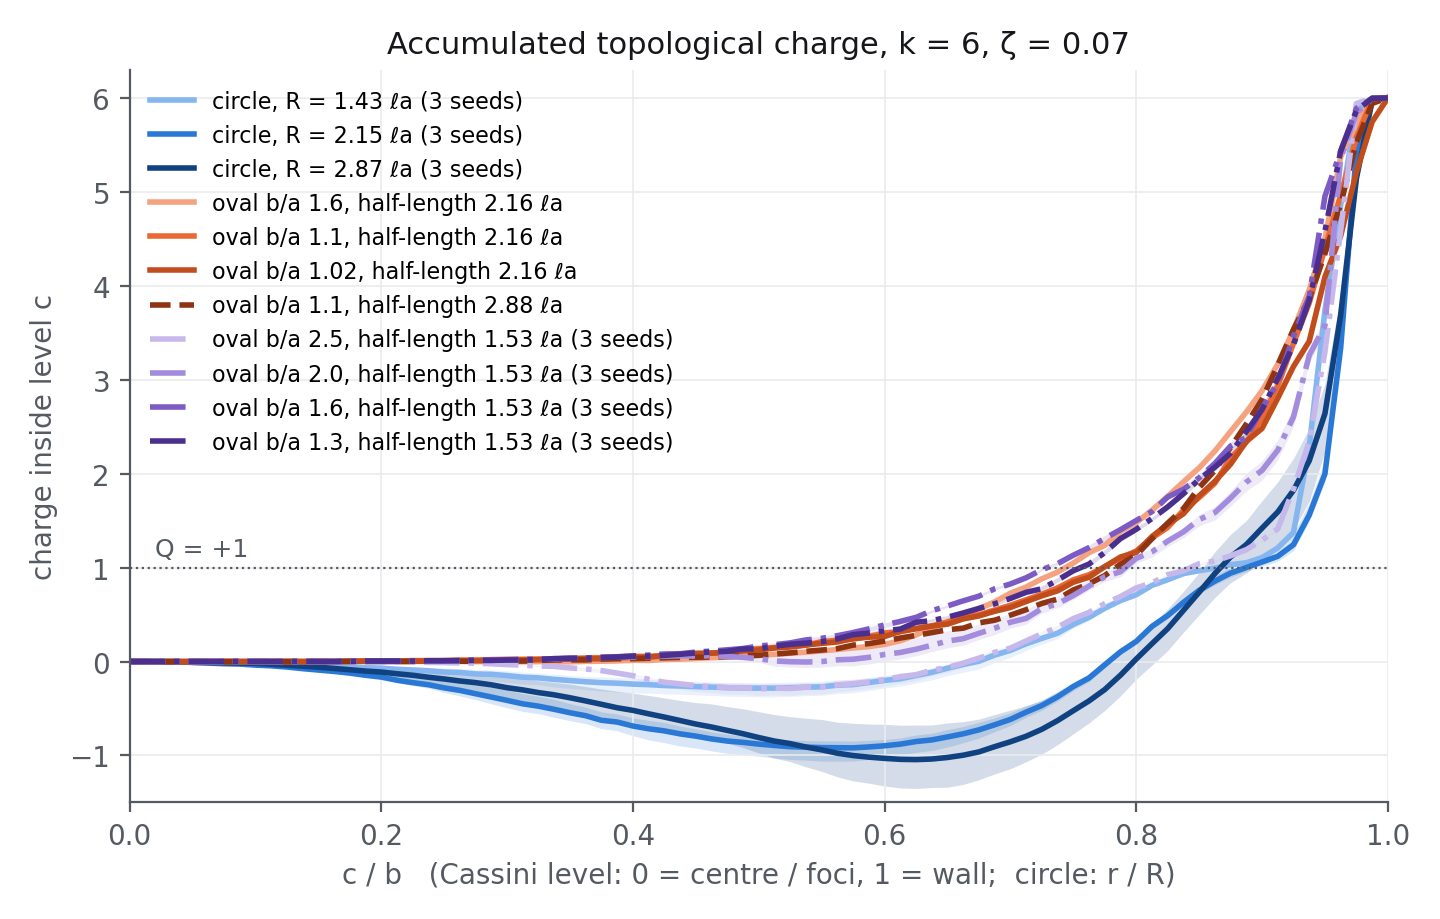
\includegraphics[width=0.85\textwidth]{figs/accumulated_charge.png}
\caption{Accumulated charge inside level $c$ ($k=6$, $\zeta=0.07$). Circles: mean of 3 seeds with min--max band. Small ovals
(half-length $1.53\,\la$, 3 seeds): dash-dotted purple, light to dark = $b/a$ 2.5 to 1.3; $b/a=2.5$ follows the circles.}\label{fig:Qc}
\end{figure}
\begin{figure}[h]\centering
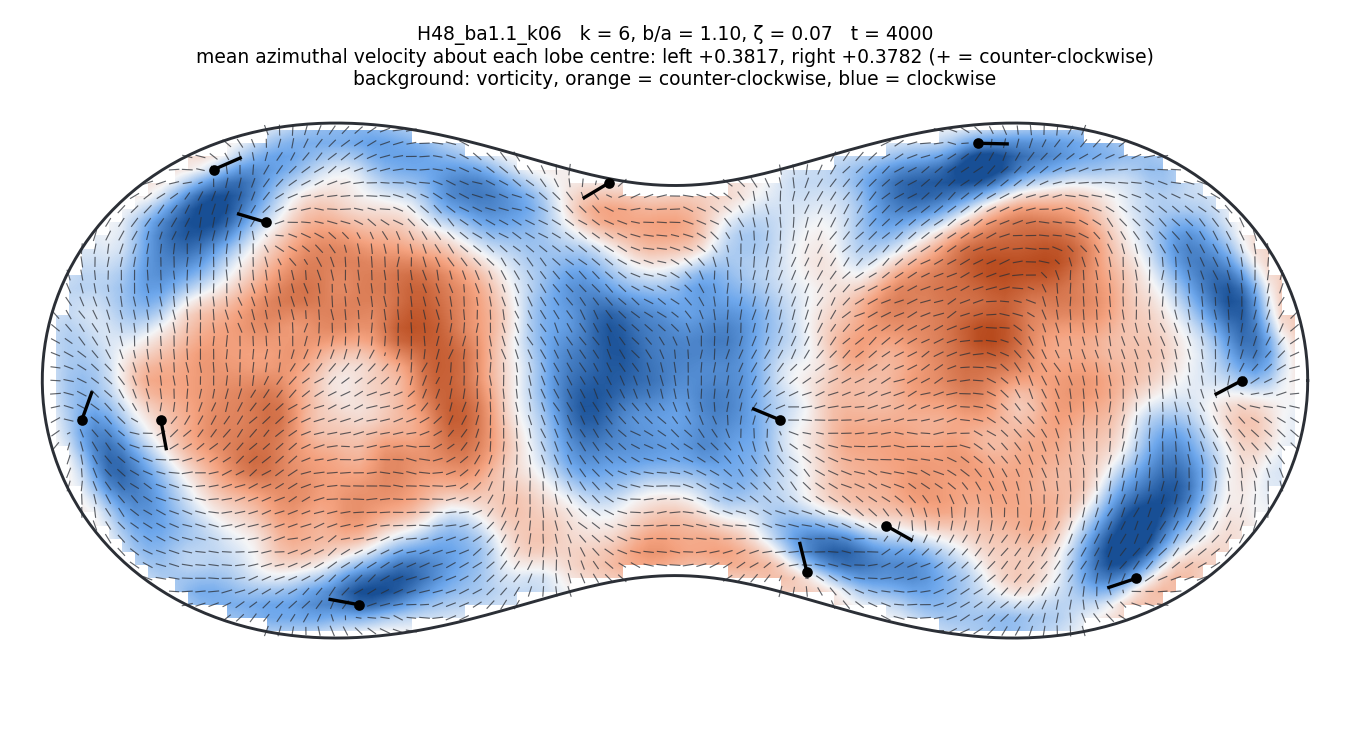
\includegraphics[width=0.49\textwidth]{figs/oval_snapshot_ba1.1.png}\hfill
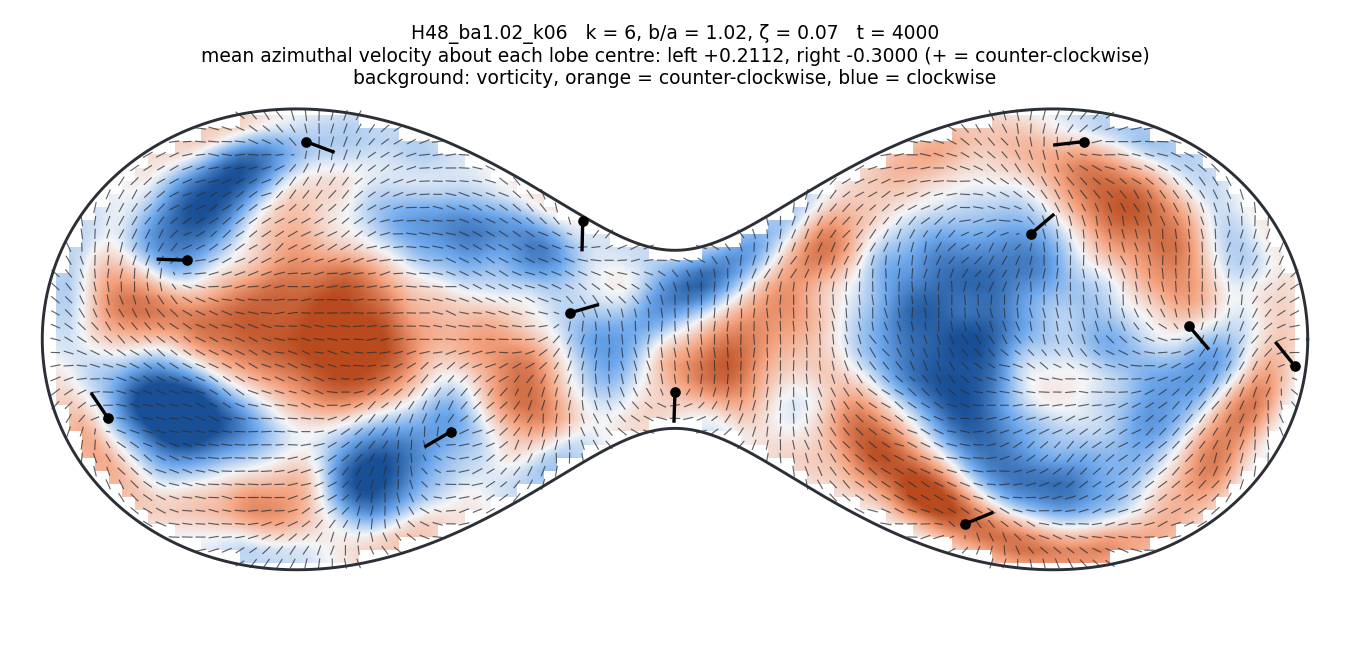
\includegraphics[width=0.49\textwidth]{figs/oval_snapshot_ba1.02.png}
\caption{Snapshots at $t=4000$: vorticity (orange counter-clockwise, blue clockwise), director, $+\frac12$ (dots with
orientation tail). Left $b/a=1.1$ (co-rotating lobes), right $b/a=1.02$ (counter-rotating).}
\end{figure}
\begin{figure}[h]\centering
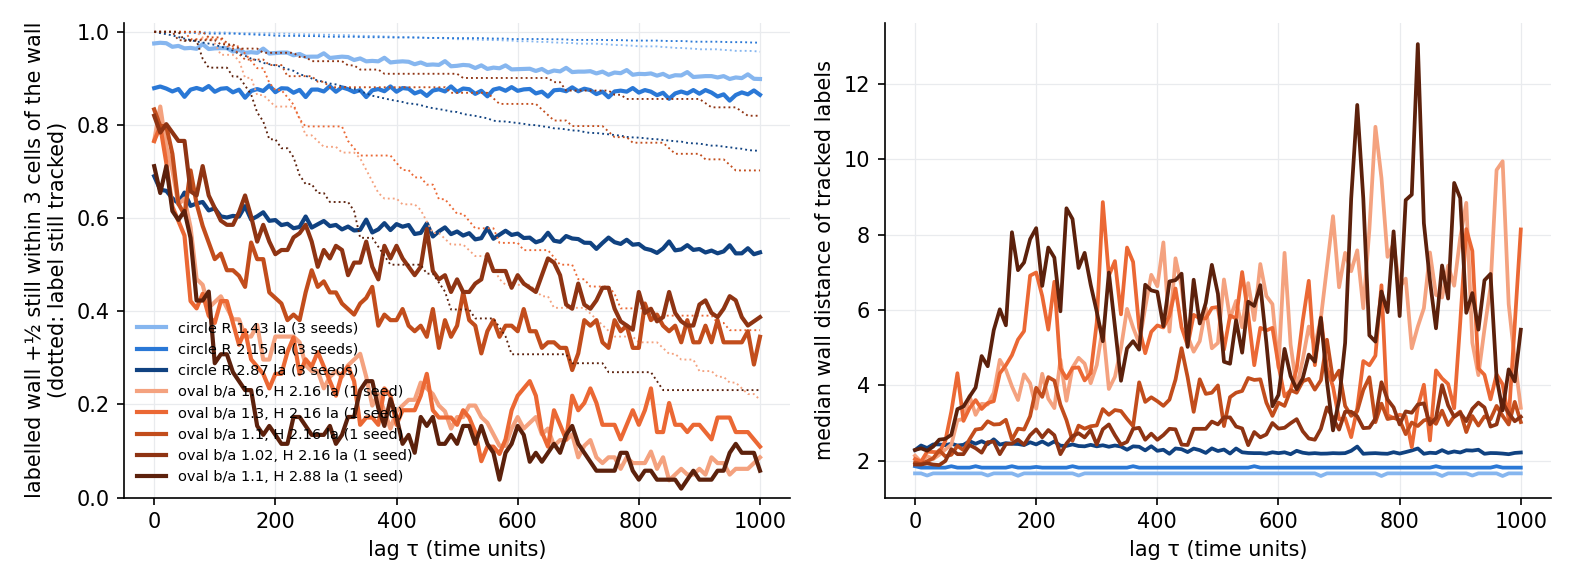
\includegraphics[width=\textwidth]{figs/bc_labels_k06.png}
\caption{Wall-defect labels followed in time (label passes to the birth partner at annihilation).
Left: fraction within 3 cells of the wall; right: median wall distance of tracked labels.}\label{fig:labels}
\end{figure}

\subsection{Size control: small ovals at half-length $1.53\,\la$}\label{sec:p3}
Four shapes ($b/a=2.5, 2.0, 1.6, 1.3$), $k=6$, 3 seeds each, at the size where circles are cleanest
(between the circles of $R=1.43$ and $1.72\,\la$). The geometric effect holds, with a sharp crossover in elongation:
\begin{table}[h]\centering\small
\caption{Small ovals (half-length $1.53\,\la$, 3 seeds) compared with circles of comparable size. Aspect = length / height.}\label{tab:p3}
\begin{tabular}{lcccccc}\toprule
cavity & aspect & sites & $q_b$ (site rule) & labels at wall after 1000 & criteria agree & $d^*/\la$\\\midrule
circle $R=1.43\,\la$ & 1 & 10 & 1.01--1.05 & 0.87--0.94 & 97--99\% & 0.19--0.20\\
oval $b/a=2.5$ & 1.17 & 10 & 1.07--1.11 & 0.82--0.86 & 97--98\% & 0.22--0.23\\
oval $b/a=2.0$ & 1.29 & 8--9 & 1.6--2.1 & 0.60--0.65 & 81--86\% & 0.29--0.31\\
oval $b/a=1.6$ & 1.5 & 13--14 & 3.3--3.5 & 0.37--0.40 & 72--74\% & 0.41\\
oval $b/a=1.3$ & 1.9 & 8--16 & 3.3--3.6 & 0.42--0.50 & 69--72\% & 0.49--0.50\\\bottomrule
\end{tabular}
\end{table}
At $b/a=2.5$ the oval is circle-like in every measure ($2k-2$ pinned sites, bulk $+1$, wall defects stay). At $b/a=2.0$
the structure is partly lost, and at $b/a\le1.6$ (still convex) it is gone. Same size, different shape, different
charge split: \textbf{the split is geometric.}

\subsection{A single number: the layer depth $d^*$}
Following B.~Loewe's suggestion: $c^*$ is where $Q(c)$ crosses $+1$ on its way to $k$, and $d^*$ the mean wall distance along
that level (circle: $R-c^*$). Normalised by $\la$ (by size, $d^*/R$ hardly changes in circles even when the layer degrades).
\begin{figure}[h]\centering
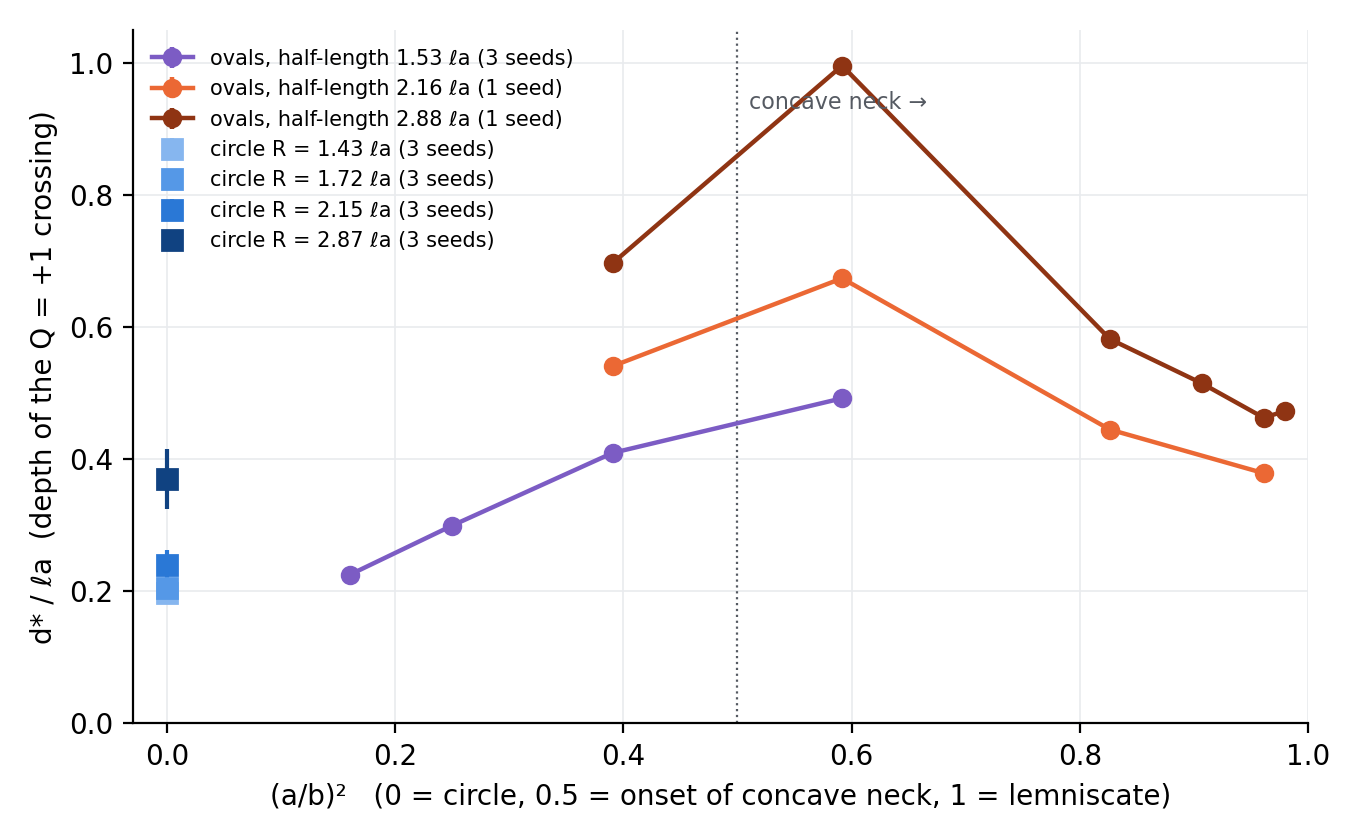
\includegraphics[width=0.82\textwidth]{figs/layer_depth.png}
\caption{Layer depth $d^*/\la$ versus elongation $(a/b)^2$ (0 circle, 0.5 onset of the concave neck, 1 lemniscate), $k=6$.
Circles 4.5--6 cells ($\approx0.2\,\la$) up to $R=2.15\,\la$. Small ovals rise from 0.23 to 0.50; larger ovals peak near
$b/a\approx1.3$.}\label{fig:dstar}
\end{figure}
See Fig.~\ref{fig:Qc} for the accumulated charge including the small ovals.

\subsection{Area fraction of the ``layer''}
Also following B.~Loewe: $f^*=A(c>c^*)/A_\mathrm{total}$, the fraction of the cavity between the $Q=+1$ level and the wall,
and the equivalent strip width $w_\mathrm{eff}=A(c>c^*)/P$. A true layer has a fixed width, so $f^*$ falls with cavity size
(circles: 0.26 at $1.43\,\la$, 0.20 at $2.15\,\la$); a charge distribution spread through the cavity gives a size-independent
$f^*$. Beyond $f^*=\frac12$ the ``layer'' would be larger than the bulk it surrounds.
\begin{figure}[h]\centering
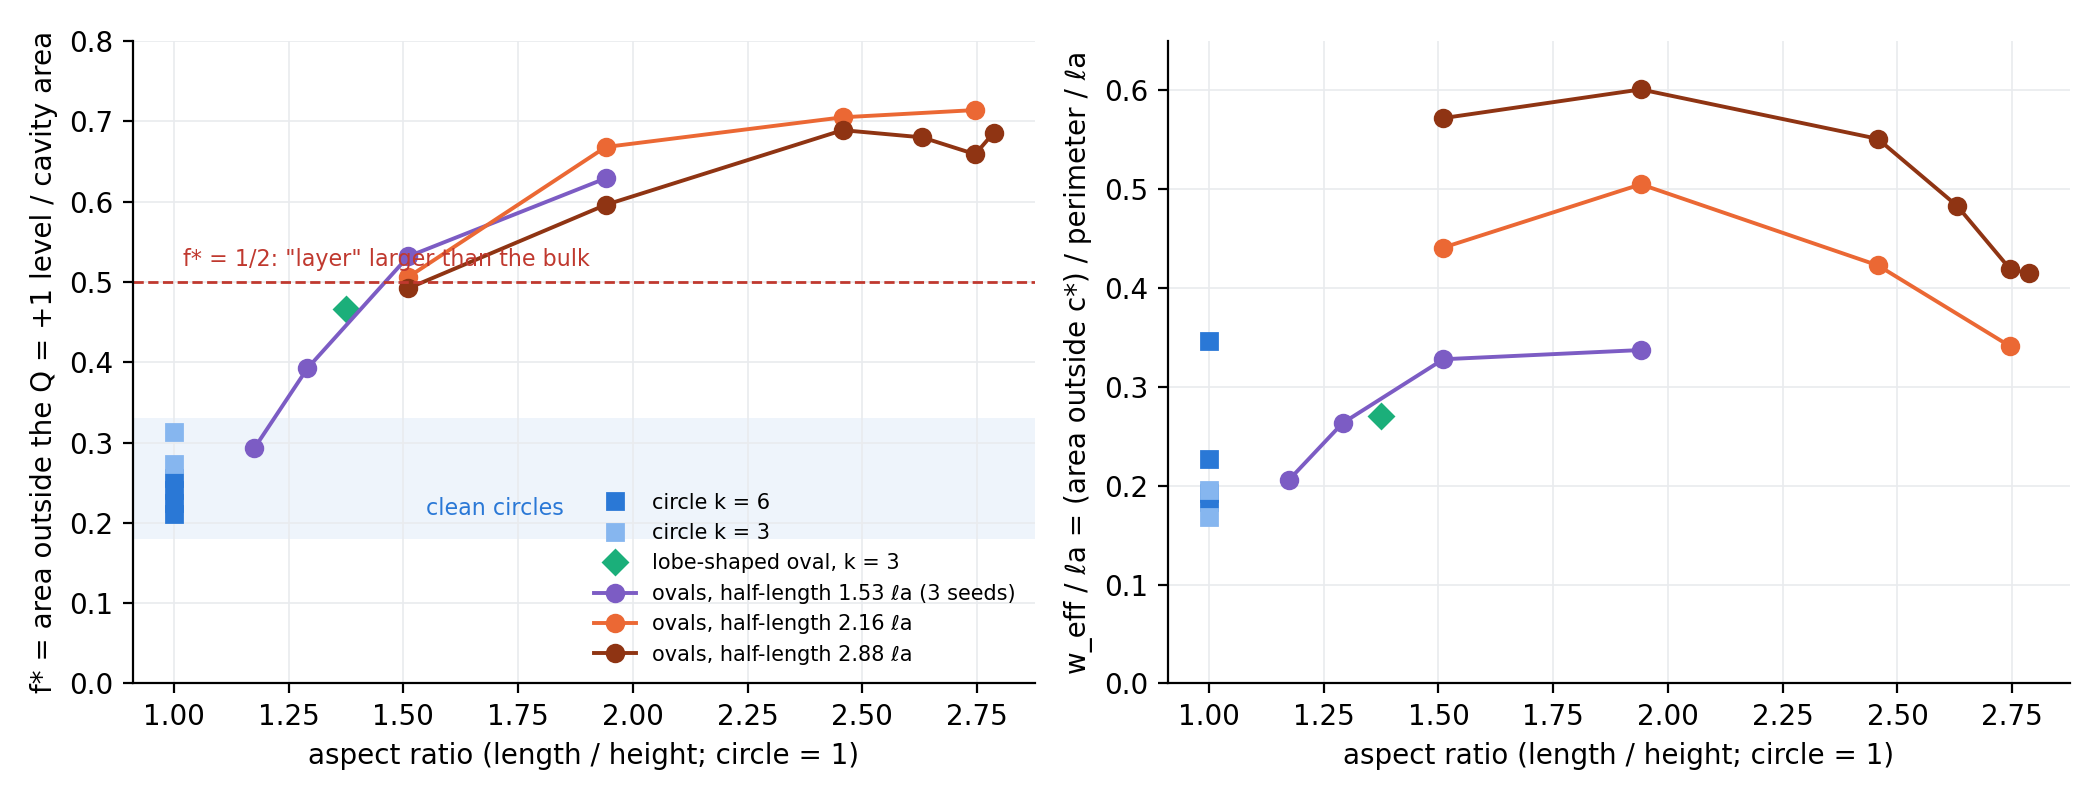
\includegraphics[width=\textwidth]{figs/layer_area.png}
\caption{Left: $f^*$ against the aspect ratio (length/height). Circles 0.20--0.32; ovals of all three sizes collapse onto
one curve (0.29 at aspect 1.17, crossing $\frac12$ near 1.5, levelling at 0.65--0.7); the lobe-shaped reference lies on it.
Right: $w_\mathrm{eff}/\la$, 0.17--0.25 for every clean circle layer, growing with size in ovals.}\label{fig:area}
\end{figure}
The collapse of $f^*$ against aspect ratio across sizes is itself the signature of ``no layer'', and identifies the
aspect ratio as the control parameter.

\subsection{Pinch-off: do the lobes become independent cavities?}
In the larger ovals $d^*$ falls again as the neck closes ($b/a\to1$). This is \textbf{not} a restored layer: in the
tightest necks ($b/a=1.01$--1.05) each lobe's charge passes $+1$ about 10 cells from the wall with slope
$\mathrm{d}Q/\mathrm{d}(c/b)\approx8$--10 (circle plateau $\approx3$), and the whole cavity passes $+2$ without a plateau.
Circles with the area of one lobe and half the winding ($k=3$, $R=23.9$ and $31.8$; server sweep, 3 seeds) keep a normal
layer ($d^*=4.1$--5.0 cells, plateau at $+1$). A lobe does not behave like a circle of its size.
\textbf{Lobe-shaped reference.} A single convex oval with the area and aspect of one lobe ($b/a=1.8$, half-length 30.4,
area 2171, aspect 1.38; $k=3$, 3 seeds) behaves like the pinched oval's lobes, not like the circle: only 3 pinned sites
(circle: $2k-2=4$), bulk $\approx1.9$ of 3, $d^*/\la=0.31$--0.32 (circles of the same area 0.18--0.22), no plateau, and
only 16--28\% of labelled wall defects at the wall after 1000 time units. \textbf{The lobe shape alone is enough to lose the
layer}; no coupling through the neck is needed. This matches the small-oval crossover: aspect 1.17 circle-like, 1.29
partial, $\ge1.38$ lost.


\subsection{Raising the winding in the pinched oval}
\begin{figure}[h]\centering
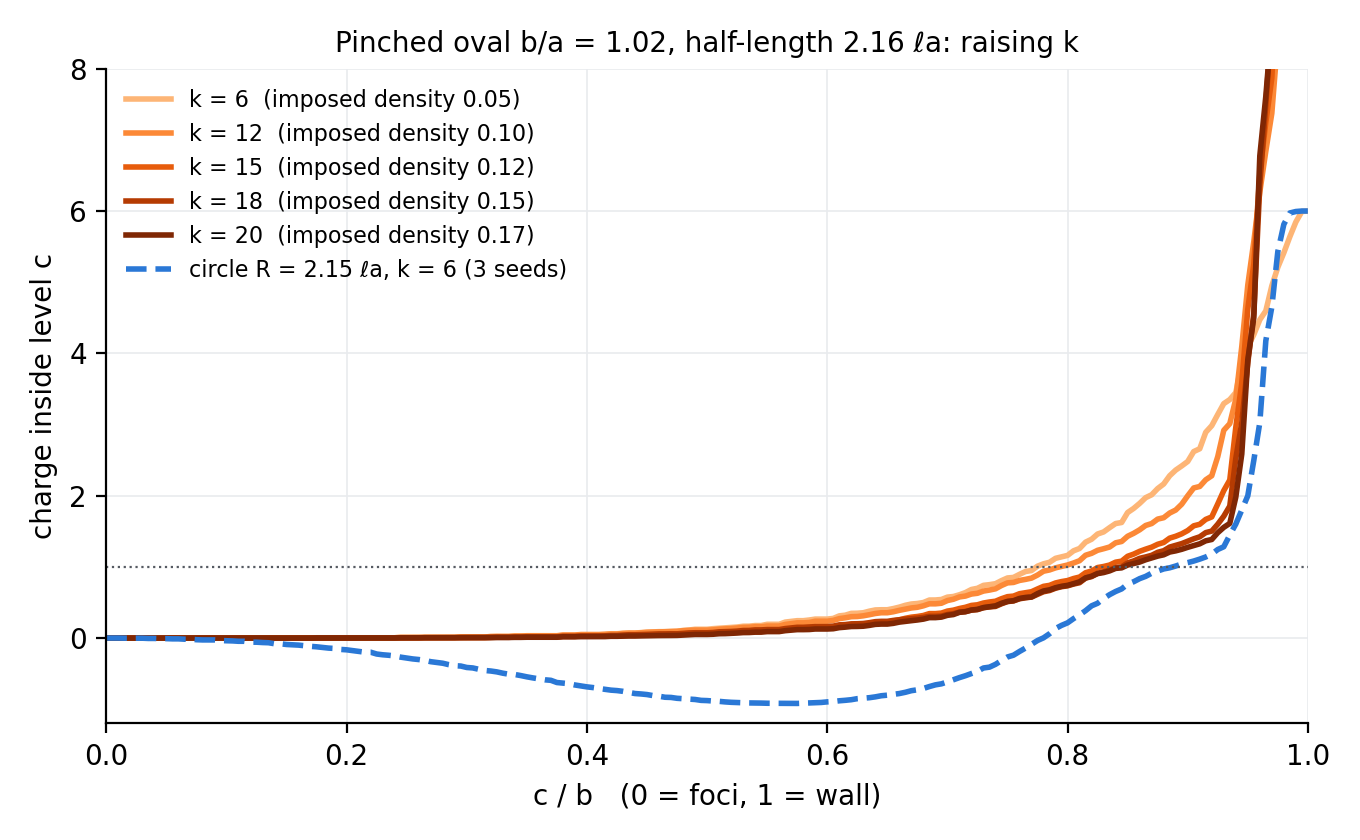
\includegraphics[width=0.82\textwidth]{figs/highk.png}
\caption{Accumulated charge in the pinched oval ($b/a=1.02$, half-length $2.16\,\la$) for $k=6$ to 20 (imposed density
0.05 to 0.17; the anchoring resolves up to $\approx0.15$), with the circle of $R=2.15\,\la$ for reference.}\label{fig:highk}
\end{figure}
A crowded wall partly restores the layer: the jump at the wall sharpens, $Q$ at $c/b=0.85$ falls from 1.76 ($k=6$) to
1.03--1.06 ($k=18$, 20), $d^*/\la$ from 0.38 to 0.30 (circle 0.20), and labelled wall defects stay at the wall (84\% after 1000
at $k=15$, 18). The bulk then carries $\approx+1$ \emph{for the whole cavity}, split as $\approx+\frac12$ per lobe, not $+1$
per lobe. So a high imposed defect density pushes the oval back towards the topological picture. $k=18$--20 is at the edge of
the anchoring resolution; 1 seed each.

\subsection{Activity $\zeta=0.09$ with three seeds}
$2k-2$ sites in all 27 runs, $q_b=1.01$--1.05, $P(q_b=+1)=0.77$--0.92, $\Phi=0.88$--0.99: the bulk charge is as clean as at
$0.07$, although the cavity centre is strongly depleted (Table~\ref{tab:dens}).


%=====================================================================
\section{Weekend 2--4 October: sweep, mirror runs, ellipses, $k$ dependence}\label{sec:weekend}

\subsection{Main sweep: where circles keep the layer}
All 1112 runs of the positive-winding sweep ($\zeta=0.07$, $k=1$--20, $\rho=0.03$--0.50, 3 seeds, plus passive references)
were analysed with the knee of $Q(r)$, the wall Fourier analysis and the site rule (Fig.~\ref{fig:diagram}).
\begin{figure}[h]\centering
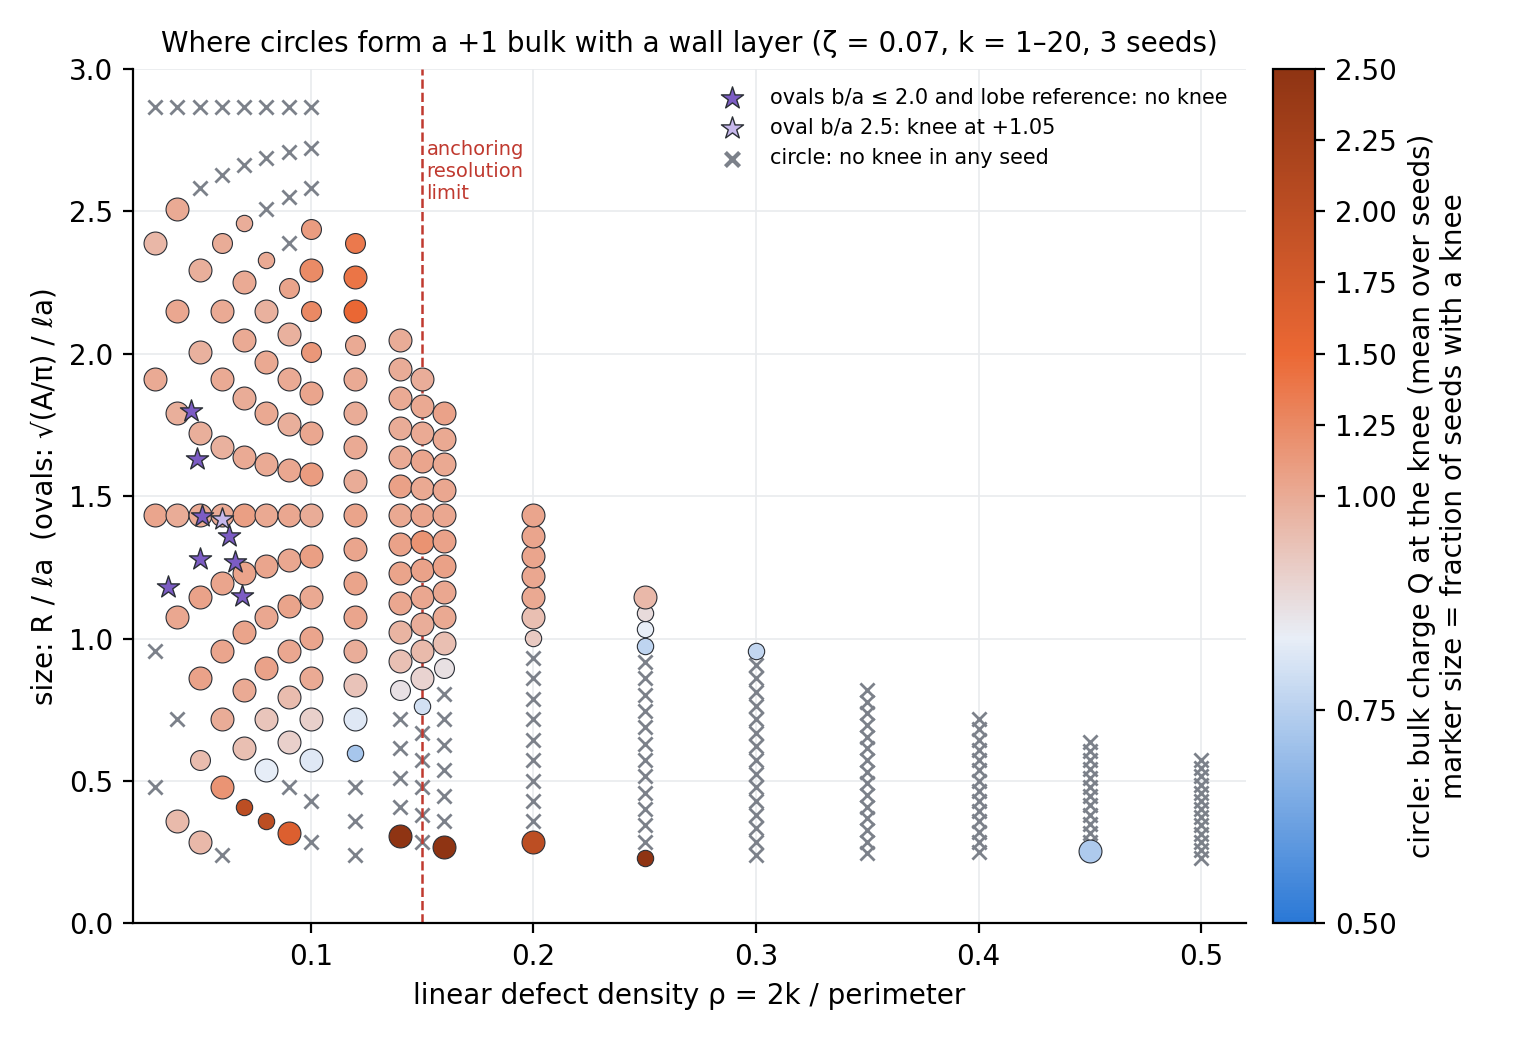
\includegraphics[width=0.85\textwidth]{figs/layer_diagram_circles.png}
\caption{Circles: bulk charge at the knee (colour; marker size = fraction of seeds with a knee; crosses: no knee) in the
plane of linear defect density $\rho=2k/P$ and $R/\la$. Stars: ovals at their own $\rho$ and equivalent radius
$\sqrt{A/\pi}/\la$.}\label{fig:diagram}
\end{figure}
\begin{itemize}
  \item For $\rho\le0.15$, circles form a $+1$ bulk with a pinned wall layer from $R\approx0.75$ to $2.0$--$2.3\,\la$, at all
        densities (knee in 89--100\% of runs, $Q_\mathrm{knee}\approx1.0$, $f_\mathrm{static}\ge0.78$). It degrades above
        $\approx2.5\,\la$ (knee in 15\%) and in very small cavities ($<0.5$--$0.6\,\la$). Beyond the resolution limit
        ($\rho\ge0.2$): mostly no knee.
  \item \textbf{Inscribed-radius test:} circles of $R=0.72$ and $0.96\,\la$ at $\rho\approx0.06$ keep a clean layer
        ($Q_\mathrm{knee}$ 1.03--1.07, $f_\mathrm{static}$ 0.97--0.98). The ovals that lose the layer have inscribed radii
        0.79--1.01\,$\la$ and $\sqrt{A/\pi}$ 1.15--1.8\,$\la$: inside the circle layer region in every size measure
        (Table~\ref{tab:match}). \textbf{The loss is a shape effect.}
  \item The knee finder needed care: the cell-quantised layer produces small steps in $Q(r)$; Q is now smoothed over
        0.045 in $r/R$ before locating the plateau.
\end{itemize}
\begin{table}[h]\centering\small
\caption{Matching ovals with circles (B.~Loewe's point 2): linear density and candidate activity numbers ($/\la$).}\label{tab:match}
\begin{tabular}{lcccccc}\toprule
cavity & $k$ & $\rho=2k/P$ & $\sqrt{A/\pi}$ & half-length & inscribed $r$ & $2A/P$\\\midrule
circle $R=1.43\,\la$ & 6 & 0.060 & 1.43 & 1.43 & 1.43 & 1.43\\
circle $R=1.07\,\la$ & 3 & 0.040 & 1.07 & 1.07 & 1.07 & 1.07\\
oval $b/a=2.5$ (H34) & 6 & 0.060 & 1.42 & 1.53 & 1.30 & 1.41\\
oval $b/a=1.6$ (H34) & 6 & 0.066 & 1.27 & 1.53 & 1.01 & 1.23\\
oval $b/a=1.3$ (H34) & 6 & 0.069 & 1.15 & 1.53 & 0.79 & 1.07\\
oval $b/a=1.6$ (H48) & 6 & 0.046 & 1.80 & 2.16 & 1.43 & 1.74\\
lobe-shaped oval & 3 & 0.036 & 1.18 & 1.37 & 1.00 & 1.16\\\bottomrule
\end{tabular}
\end{table}

\subsection{Mirror runs (H5): the bulk stays positive}
570 runs with winding $-|k|$ (Fig.~\ref{fig:mirror}). $Q(r)$ rises to a \emph{positive} peak before plunging to $-|k|$ at the
wall: the bulk charge is positive, not $-1$, and grows with $|k|$: 0.09 ($|k|=2$), 0.47 (6), 0.83 (10), 1.00--1.02
($|k|=15$--20); the wall carries $\approx2|k|+2\,q_b$ of the $-\frac12$ defects. At fixed size the bulk charge rises with
$|k|$; at fixed $|k|$ it peaks at $R\approx1.5$--$2\,\la$.
\textbf{$+1$ (the Euler characteristic) is the attractor for both winding signs, but activity breaks the mirror symmetry:}
with $+k$ the $+1$ bulk appears at every $k\ge2$ (made of self-propelled $+\frac12$); with $-k$ the wall has to absorb two
extra $-\frac12$, which happens fully only for $|k|\gtrsim13$--15.
\begin{figure}[h]\centering
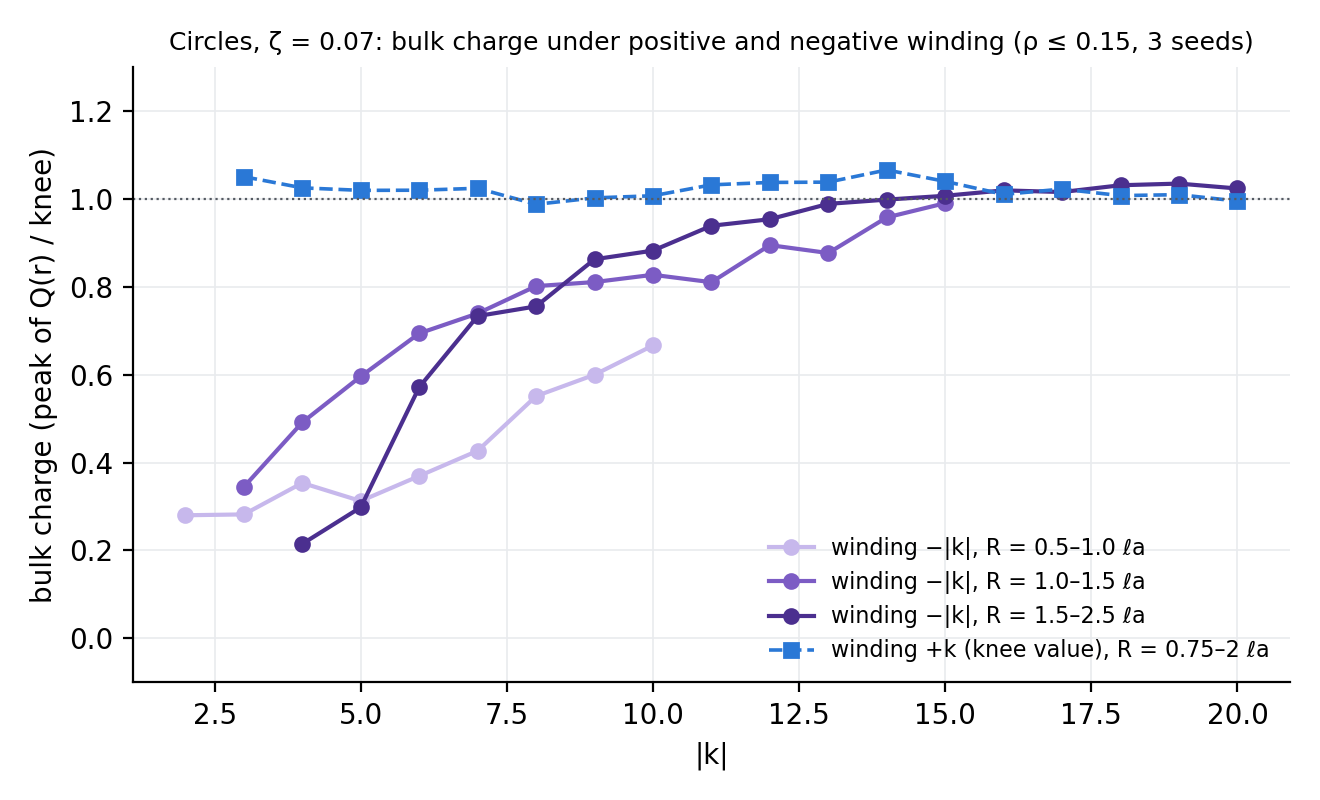
\includegraphics[width=0.8\textwidth]{figs/mirror_bulk_vs_k.png}
\caption{Bulk charge versus $|k|$: positive winding (knee value, squares) and negative winding (peak of $Q(r)$, three size
bins).}\label{fig:mirror}
\end{figure}

\subsection{Shape: size collapse with seeds, and ellipses}
\begin{figure}[h]\centering
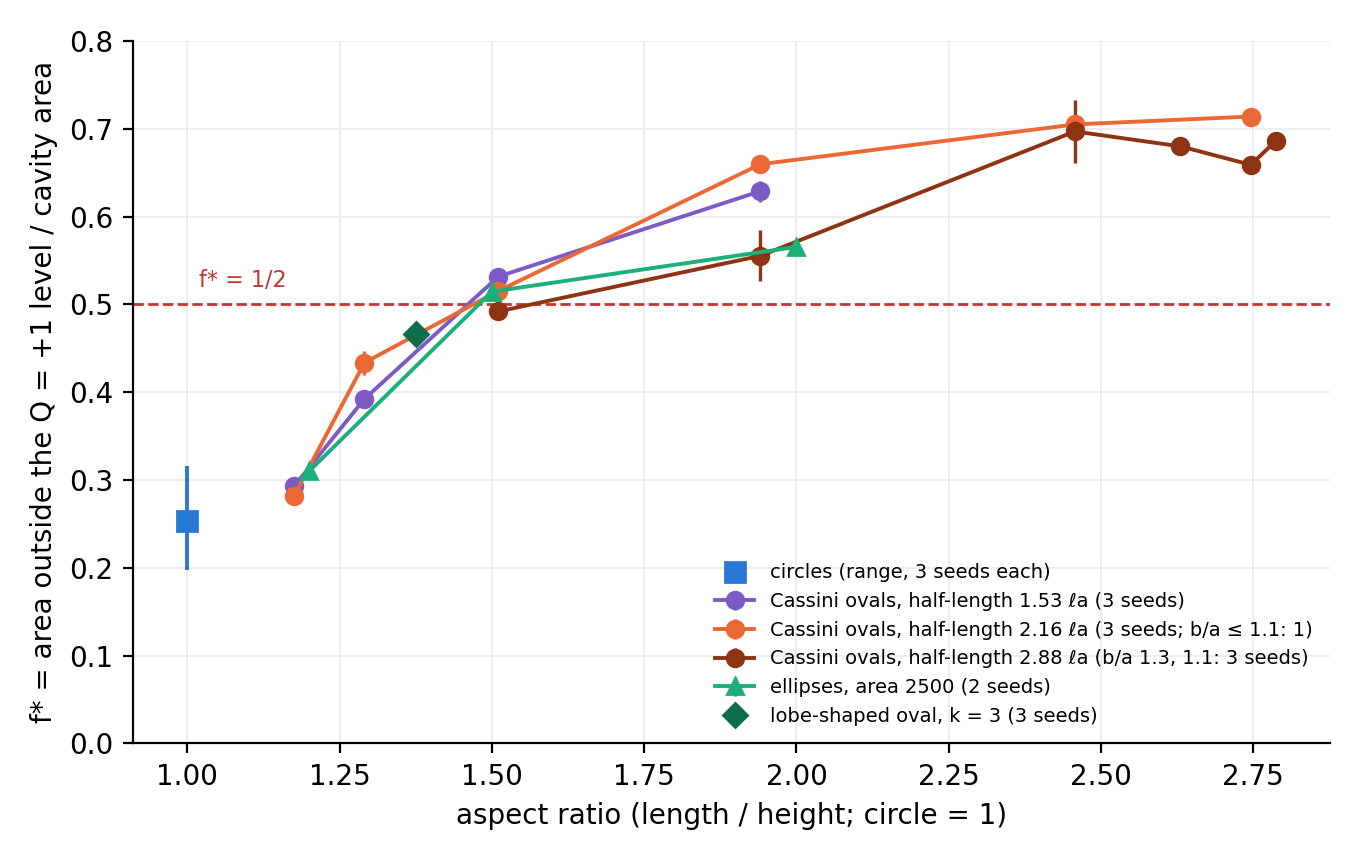
\includegraphics[width=0.85\textwidth]{figs/layer_area_all.png}
\caption{Area fraction outside the $Q=+1$ level versus aspect ratio, all shapes with seeds: Cassini ovals at three sizes,
ellipses (area 2500), the lobe-shaped reference, circles.}\label{fig:areaall}
\end{figure}
\begin{itemize}
  \item \textbf{Size collapse confirmed with seeds:} $f^*$ at half-length 34 / 48 ($1.53$ / $2.16\,\la$): $b/a=2.5$: 0.29 / 0.28;
        2.0: 0.39 / 0.42--0.45; 1.6: 0.53 / 0.49--0.54; 1.3: 0.63 / 0.65--0.67. At $2.88\,\la$ (3 seeds for $b/a$ 1.3, 1.1) slightly
        lower ($\approx0.56$ at aspect 1.94).
  \item \textbf{Ellipses fall on the same curve} (B.~Loewe's question: can a convex cavity lose the layer? \emph{Yes}):
        aspect 1.2: knee 0.98--1.07, $f^*=0.31$, pinned lattice; 1.5: no knee, $f^*=0.51$--0.52; 2.0: no knee, $f^*=0.57$.
        Elongation (aspect $\gtrsim1.4$--1.5) is the generic control for both convex families.
\end{itemize}

\subsection{Dependence on the winding $k$ (B.~Loewe's point 1)}
Half-length 34, $b/a$ 2.0 and 1.6, $k=2\dots12$, 3 seeds. Measured by $Q$ at a fixed depth (no knee needed):
\begin{table}[h]\centering\small
\caption{$Q(c/b=0.85)$ versus $k$ (mean of 3 seeds); knees found (seeds) in brackets.}
\begin{tabular}{lcccccc}\toprule
& $k=2$ & 4 & 6 & 8 & 10 & 12\\\midrule
circle $R=1.43\,\la$ & 0.99 & 0.95 & 0.95 & 0.94 & 0.97 & --\\
oval $b/a=2.0$ & 1.12 & 1.54 & 1.51 & 1.49 & 1.36 & 1.24 (3/3, 1.31)\\
oval $b/a=1.6$ & 1.30 & 2.06 & 1.96 & 1.63 & 1.42 (1/3) & 1.31 (3/3, 1.40)\\\bottomrule
\end{tabular}
\end{table}
The circle is a \emph{traditional} layer ($Q$ at fixed depth independent of $k$). The ovals are neither traditional nor
``all winding into the bulk'': the bulk carries a bounded excess (at most $\approx+1$) at moderate $k$, which shrinks again
as the wall gets crowded; at $k=12$ ($\rho\approx0.13$) a plateau and a wall lattice reappear ($f_\mathrm{static}$ for
$b/a=1.6$: 0.03, 0.21, 0.11, 0.39, 0.70 for $k=2\dots12$). Same trend as the high-$k$ pinched oval and the mirror runs:
\textbf{a crowded wall restores the topological structure}; elongation matters most at moderate imposed density.

\subsection{New layer measures (B.~Loewe's points 1, 3, 4)}
\begin{itemize}
  \item \textbf{Knee of $Q(c)$}: bulk charge from the plateau, no assumption that it is $+1$. Clean circles and the $b/a=2.5$ oval:
        1.0--1.1; elongated ovals and ellipses: no knee. No ``less-charged layer'' (plateau at $+2$, $+3$) in the clean regime;
        large circles at high $k$ ($\rho\approx0.1$--0.12, $R\approx2$--$2.6\,\la$) show a tilted plateau at 1.3--2.1 (to check).
  \item \textbf{Wall Fourier analysis} (density along the wall arclength): instantaneous structure factor $S(m)$, static fraction
        $f_\mathrm{static}=|\langle\rho_m\rangle|^2/\langle|\rho_m|^2\rangle$. Pinned lattice (circles, $b/a=2.5$, ellipse 1.2):
        peak at $m=2k-2$, $S\approx8$--9, $f\approx0.97$--0.99; large circle (2.87\,$\la$): $f=0.87$ (partly sliding);
        elongated ovals and ellipses: $S\approx1.5$--2.7, $f\approx0$--0.4 (no lattice).
  \item \textbf{Heat maps} of the defect positions for all shapes (in the analysis folders).
\end{itemize}

\subsection{Wall--bulk exchange (H7)}
From gap-closed tracks (89--96\% of track ends paired as $\pm\frac12$ events): escape rate of wall $+\frac12$ (per
$10^3$ time units) and mean residence: circles 0.3--0.5 / 900--2000; large circle (2.87\,$\la$) 4.5 / 220; oval $b/a=2.5$
0.7 / 730--970; 2.0: 2.7--3.4 / 200--250; 1.6, 1.3: 5.5--6.2 / 140--150; lobe reference 7.6 / 125. Wall defects in
elongated cavities escape 10--20$\times$ faster; $\le10\%$ of wall visits end in annihilation (the layer empties by undocking).

\subsection{Server}
Sweep complete (1304/1304 on 3 Oct, 0 failures). The \texttt{cassini} branch binary is built and validated on the server
(circle and $a=0$ oval match the production binary). An oval sweep is \textbf{drafted, not launched}
(\texttt{reports/oval\_sweep\_draft.md}): 9 shapes $\times$ 3 equivalent sizes $\times$ 4 densities $\times$ 3 seeds = 324 runs,
$\approx1.2$ days; open choices (mirror subset, high-$\rho$ column, ellipses) listed there.


%=====================================================================
\section{Monday 5 October: flow, wall lattice dynamics, edge criteria}\label{sec:monday}

\subsection{Flow and wall-defect tilt in circles}
Per-frame flow reduction of 930 circle runs ($\rho\le0.15$, $\pm k$, 3 seeds) on the server (Fig.~\ref{fig:flow}).
\begin{itemize}
  \item The mean azimuthal flow $|\langle v_\theta\rangle|$ collapses on $R/\la$ for all $\rho$: $\approx0.35$ at $0.6\,\la$,
        0.9--1.0 at 2--2.5\,$\la$ (Mach $\sim1$). The circulation fraction is 0.8--0.9 between 0.5 and $2.5\,\la$; for $+k$
        it collapses to 0.2--0.4 (reversals) above $\approx2.5\,\la$, the same size where the layer is lost. No coherent
        vortex below $0.4\,\la$.
  \item Enstrophy peaks ($\approx0.01$--0.015) at $R\approx0.4$--$0.5\,\la$ and decays to 0.004 at $2.9\,\la$; $+k$ exceeds
        $-k$ by 20--30\% below $2\,\la$.
  \item Wall $+\tfrac12$ lean downstream by 60--65$^\circ$ at $\rho\le0.06$, 30--40$^\circ$ at $\rho=0.14$--0.15; the tilt
        vanishes where the layer is lost. Wall $-\tfrac12$ lean downstream by 8--15$^\circ$. The tilt sign agrees with the
        circulation in $\approx100\%$ of frames inside the layer window.
\end{itemize}
\begin{figure}[h]\centering
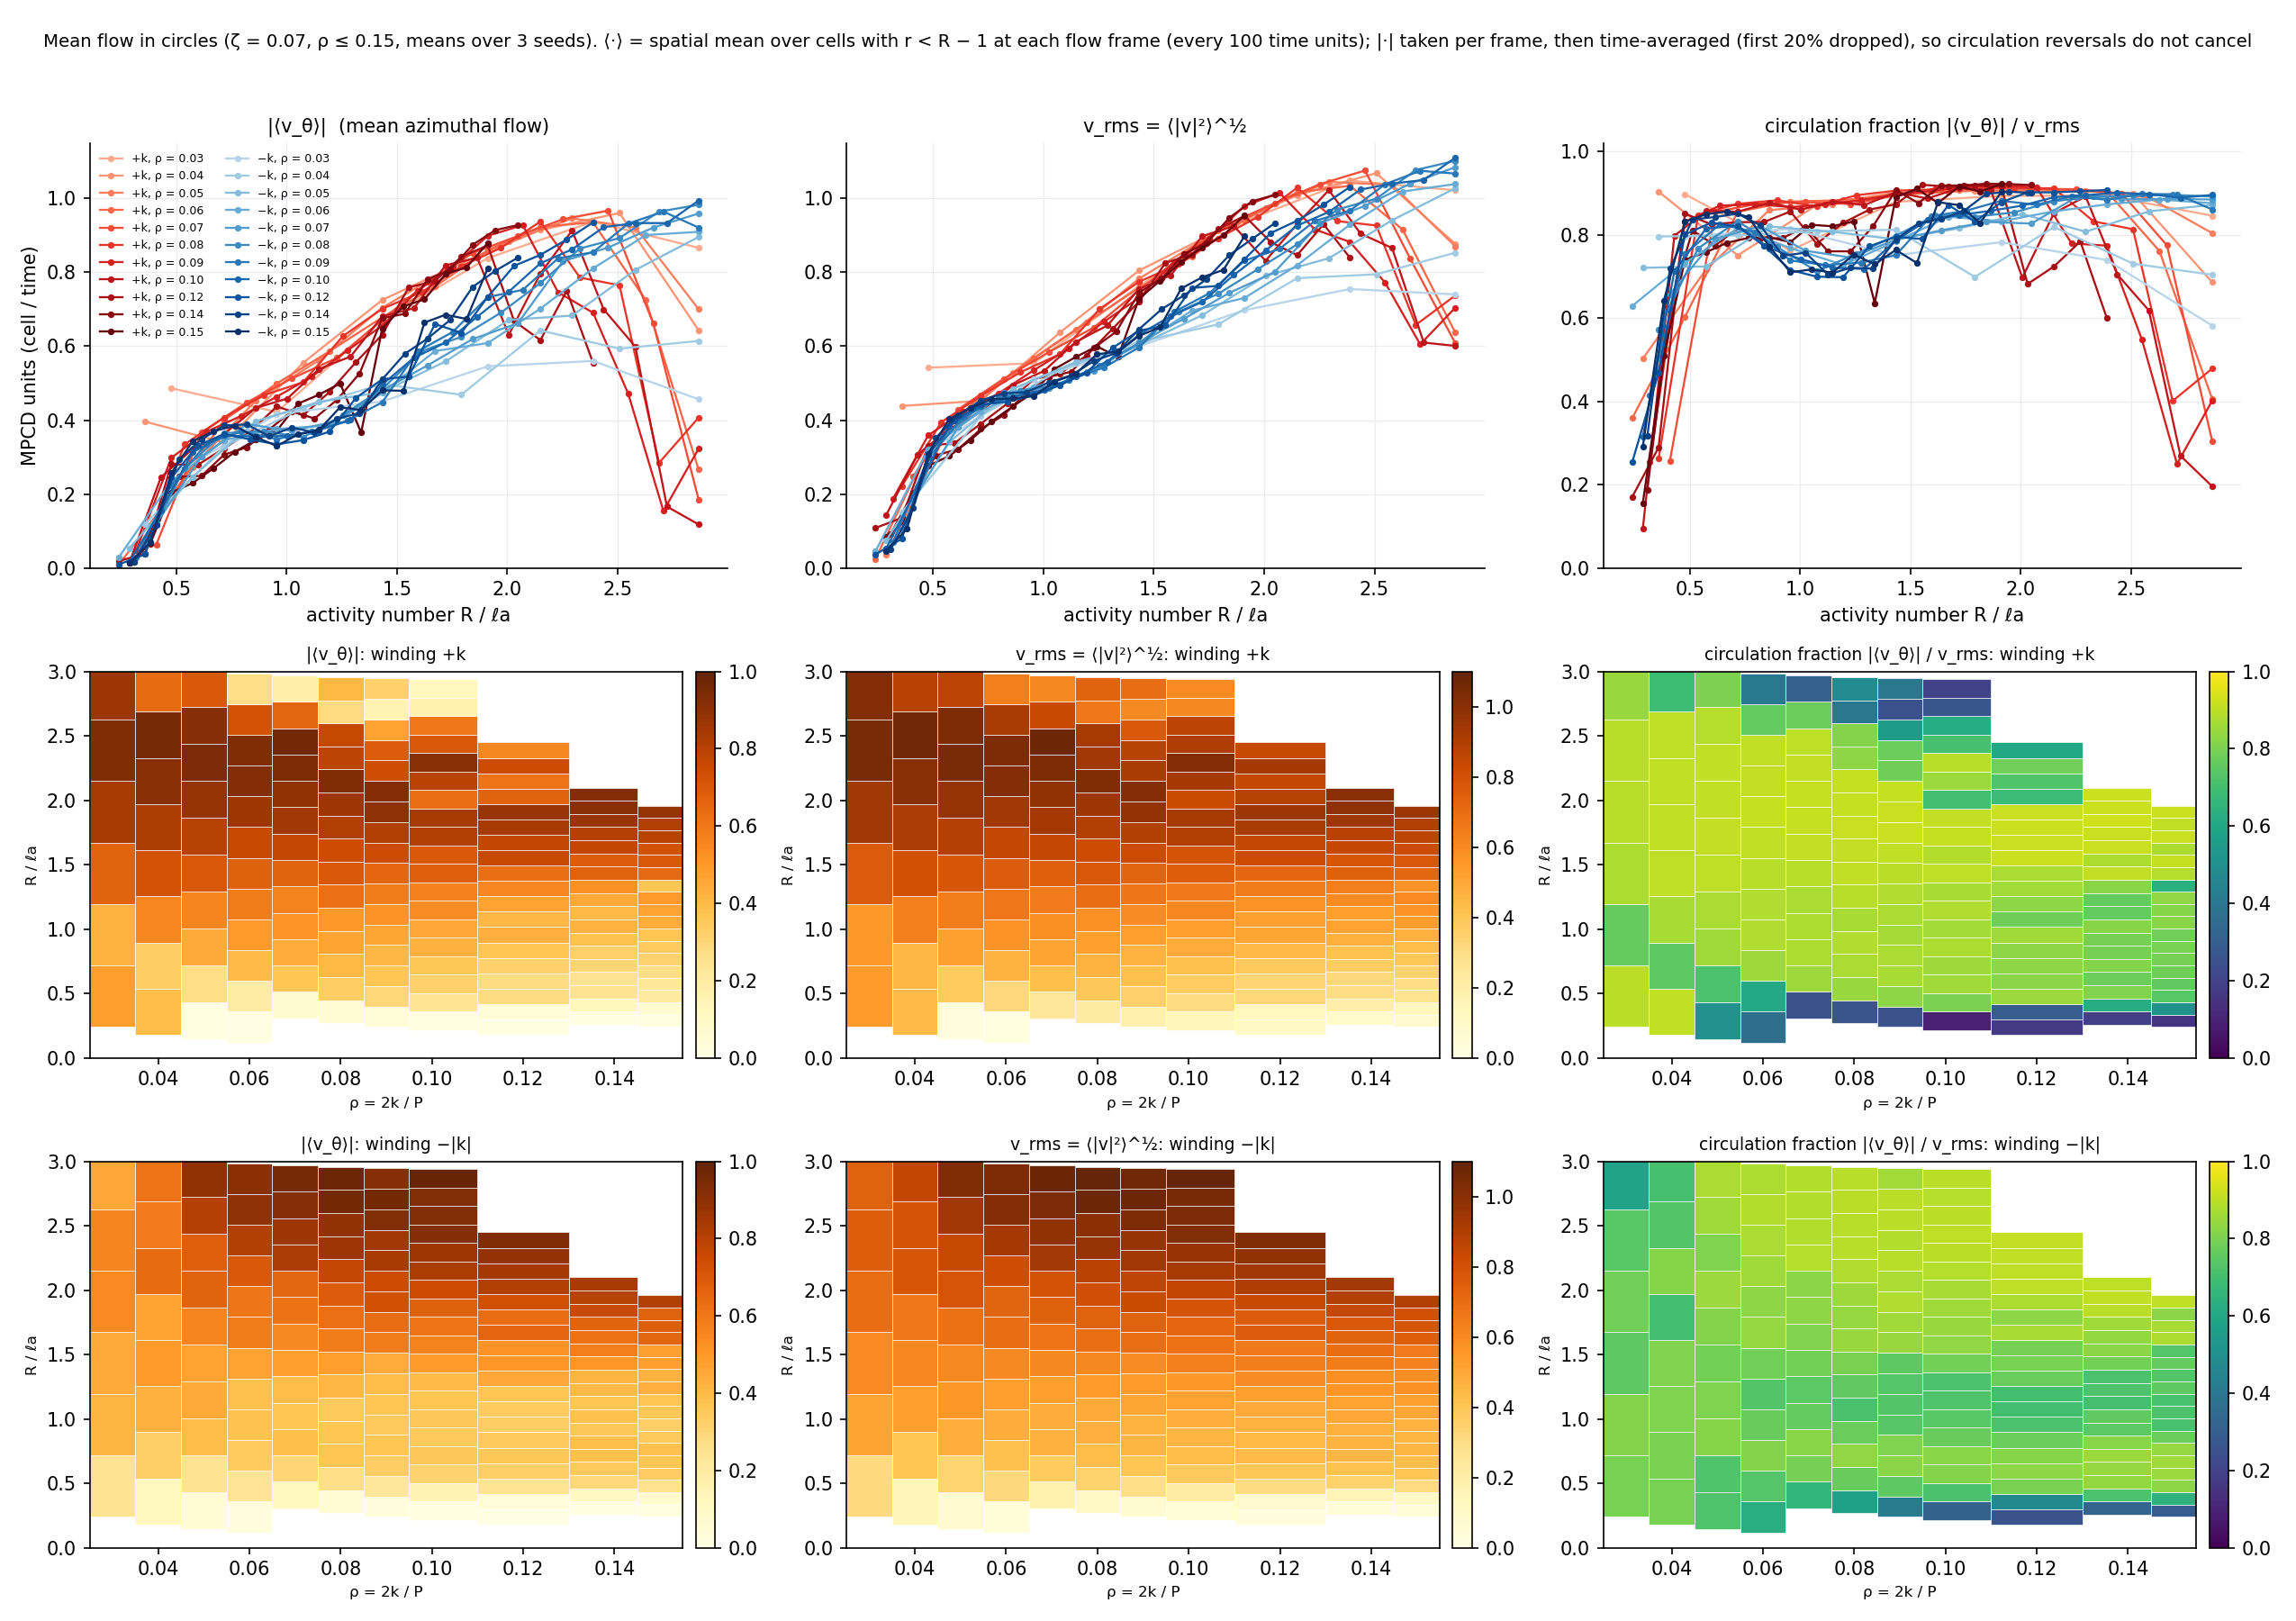
\includegraphics[width=\textwidth]{figs/flow_mean.png}\\[1ex]
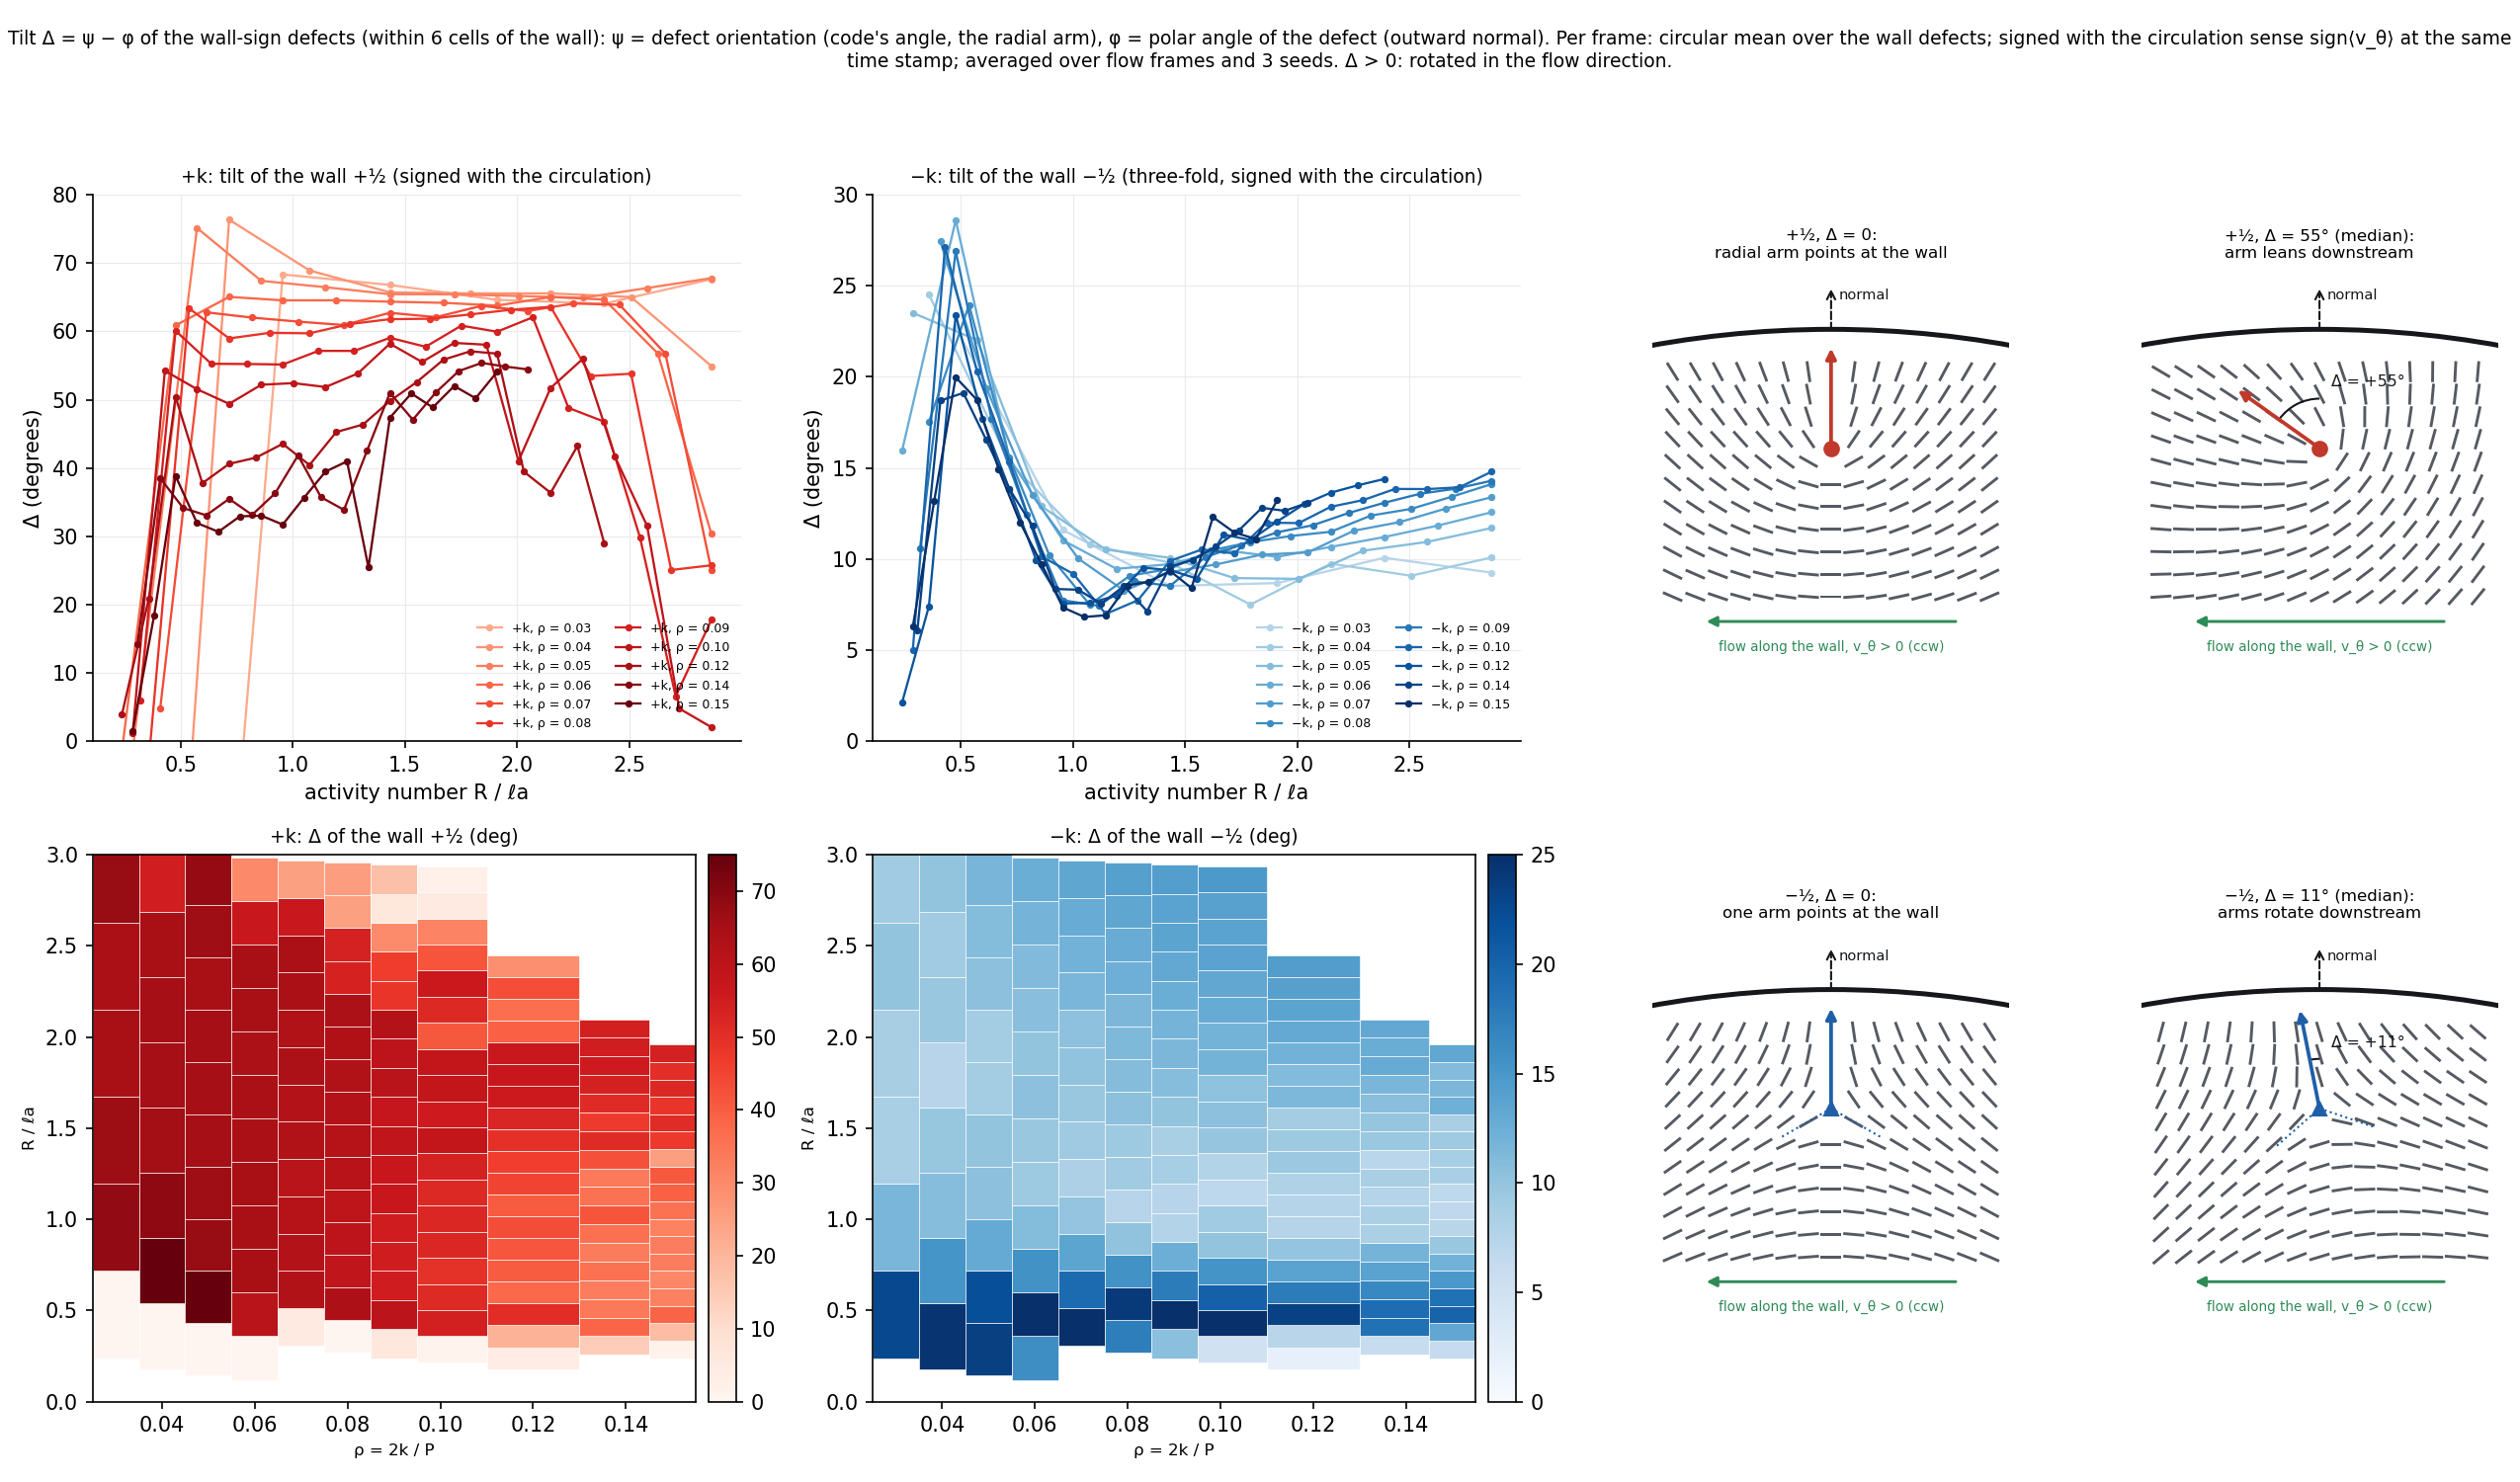
\includegraphics[width=\textwidth]{figs/flow_tilt.png}
\caption{Circles: mean flow and circulation (top) and wall-defect tilt (bottom) vs $R/\la$ and $\rho$.}\label{fig:flow}
\end{figure}

\subsection{Wall Fourier analysis for all circles}
Static and dynamic Fourier modes of the wall-sign defects along the wall (Figs.~\ref{fig:fourier-static},
\ref{fig:fourier-dyn}).
\begin{itemize}
  \item The lattice period is that of a $+1$ bulk for both windings ($2k-2$ for $+k$, $2|k|+2$ for $-k$) wherever
        $R\gtrsim0.5$--$0.75\,\la$.
  \item \textbf{Mirror runs:} the $-\tfrac12$ wall lattice has the $+1$-bulk period but is under-occupied (0.7--0.9 at low
        $\rho$, $\to1$ at high $\rho$ or large $|k|$). These vacancies are why the mirror bulk stays below $+1$; the bulk charge
        from the wall count tracks the slow-defect criterion ($r=0.96$).
  \item $+k$: full occupancy from 0.75 to $2.3\,\la$, dropping to 0.6--0.85 above $2.5\,\la$; $f_\mathrm{static}\approx0.95$--1.
  \item \textbf{No steady sliding anywhere:} lattice speed $<2$--3\% of $|\langle v_\theta\rangle|$ for $R>0.6\,\la$. The
        ``ordered but sliding'' class never appears: the layer is pinned, or vacant and melting.
\end{itemize}
\begin{figure}[h]\centering
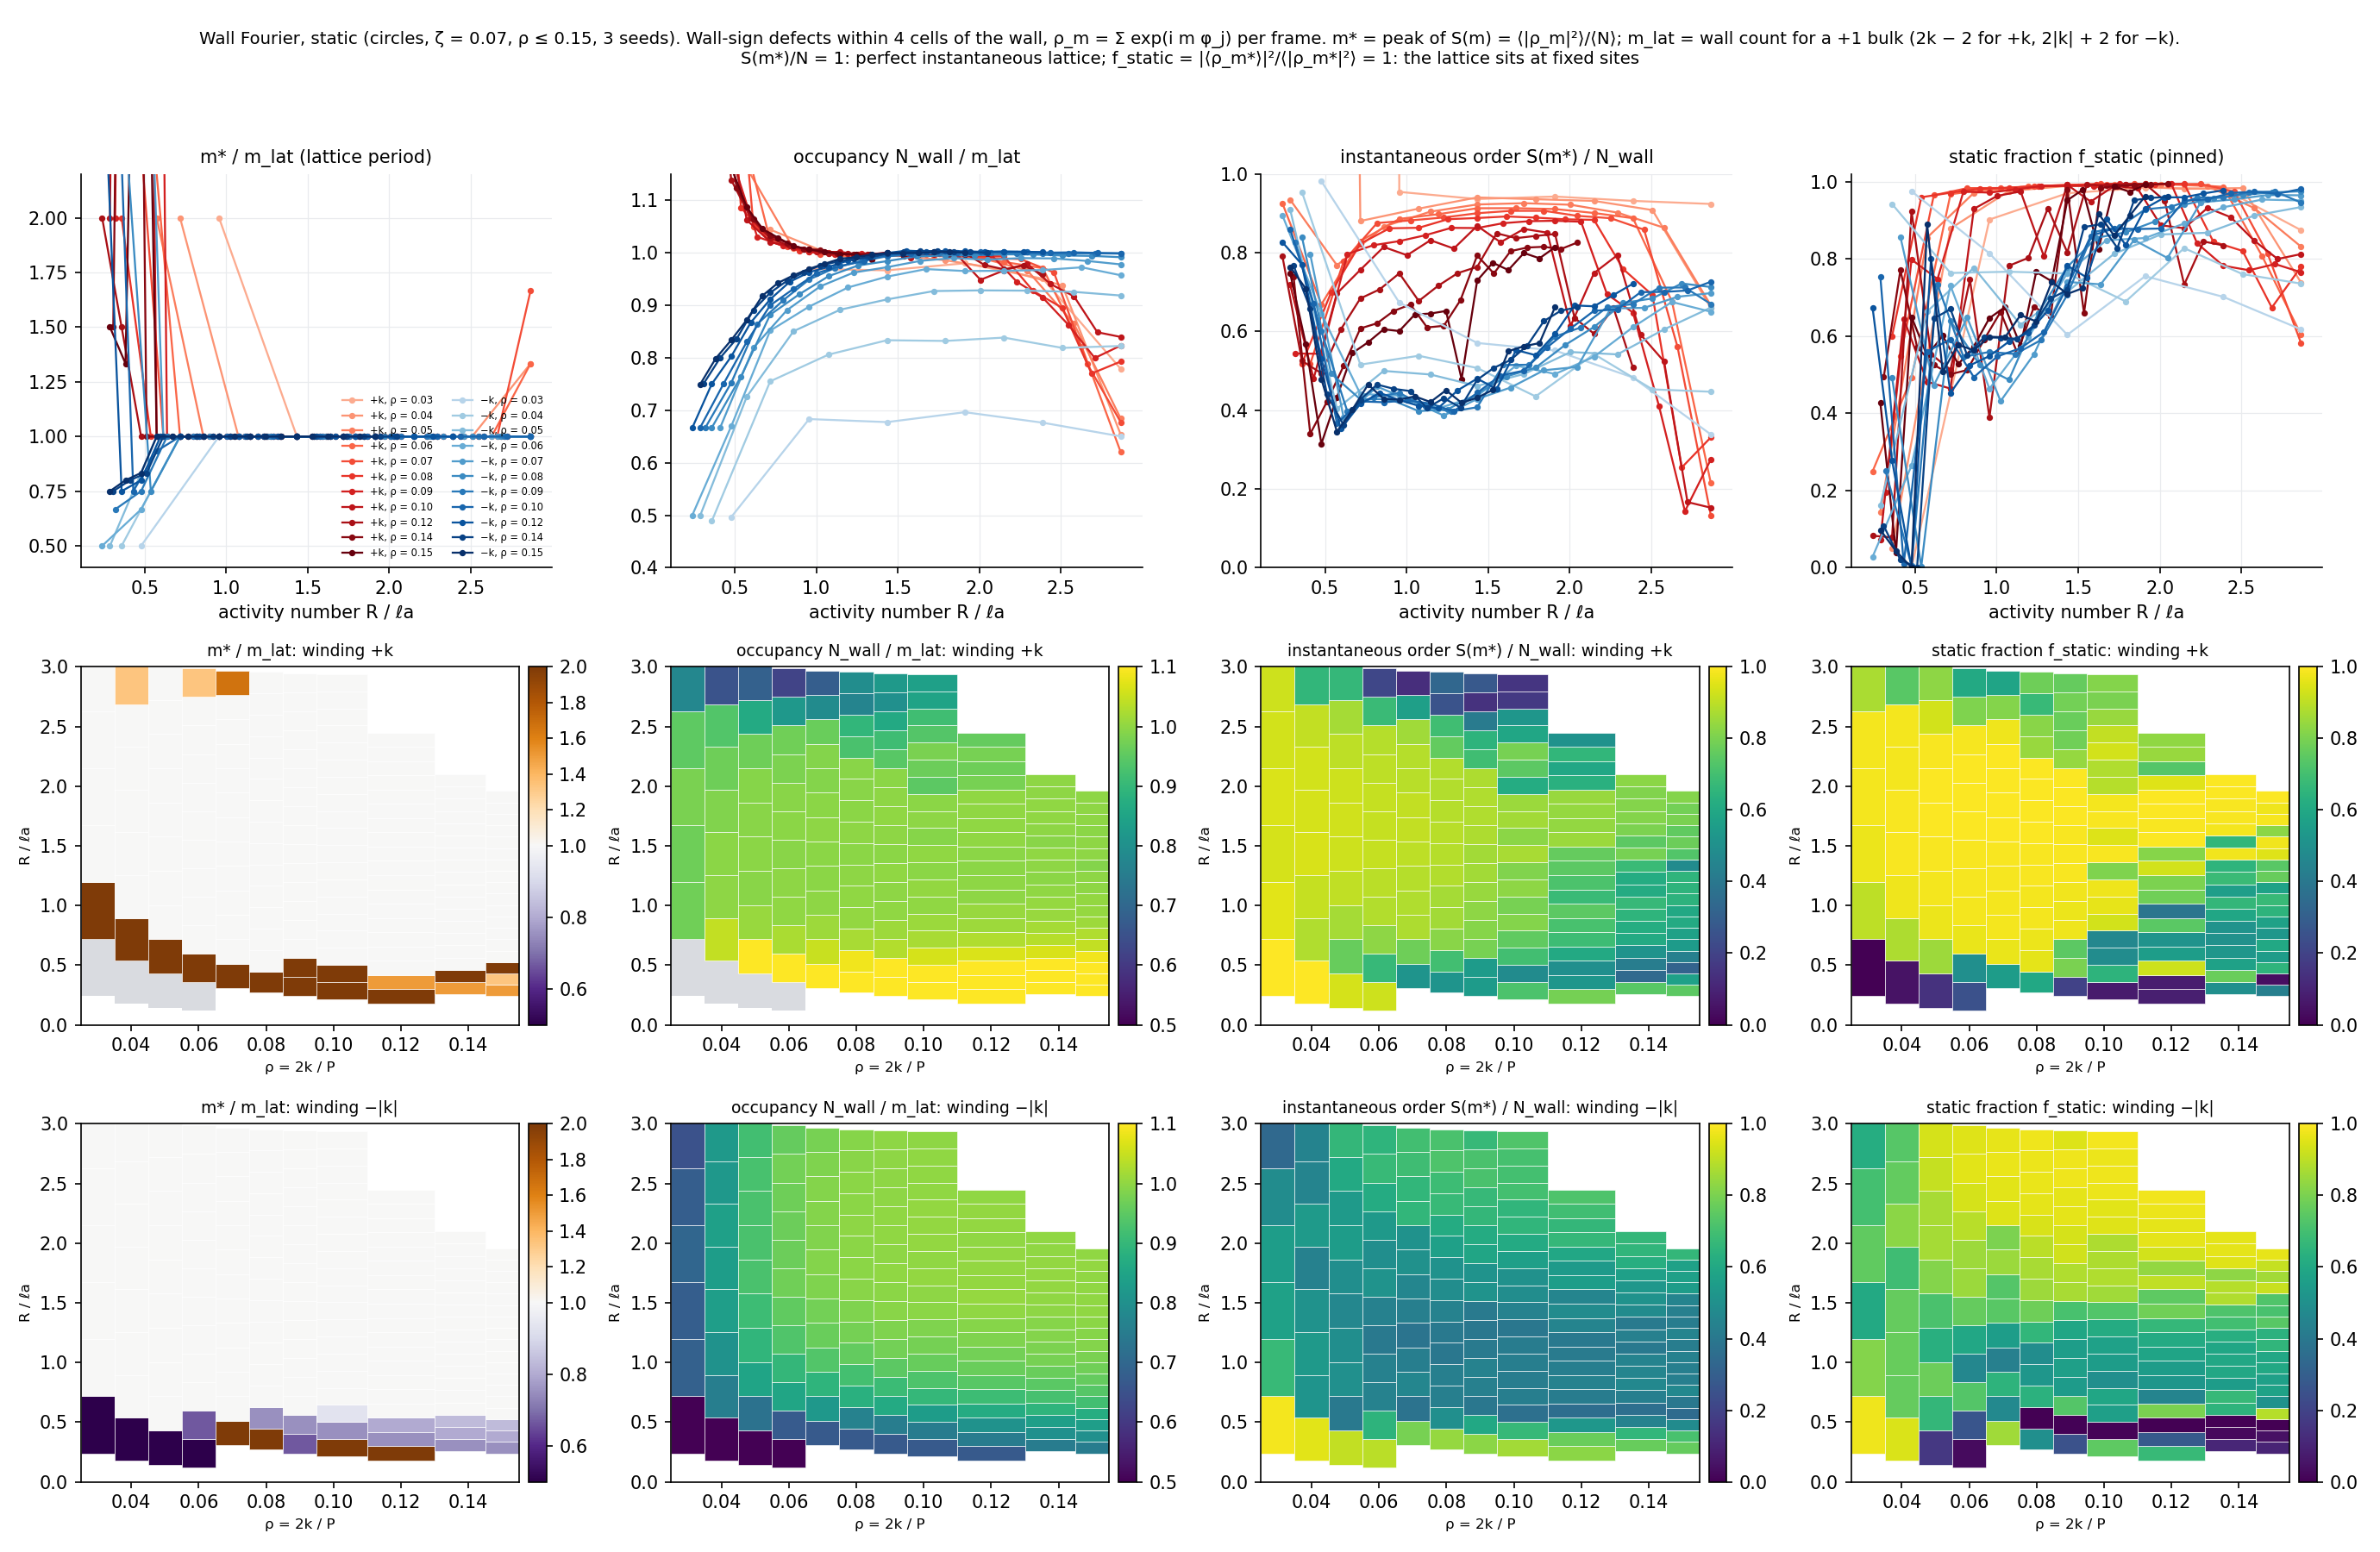
\includegraphics[width=\textwidth]{figs/fourier_static_circles.png}
\caption{Circles, static wall Fourier: lattice period, occupancy, instantaneous order and static fraction.}\label{fig:fourier-static}
\end{figure}
\begin{figure}[h]\centering
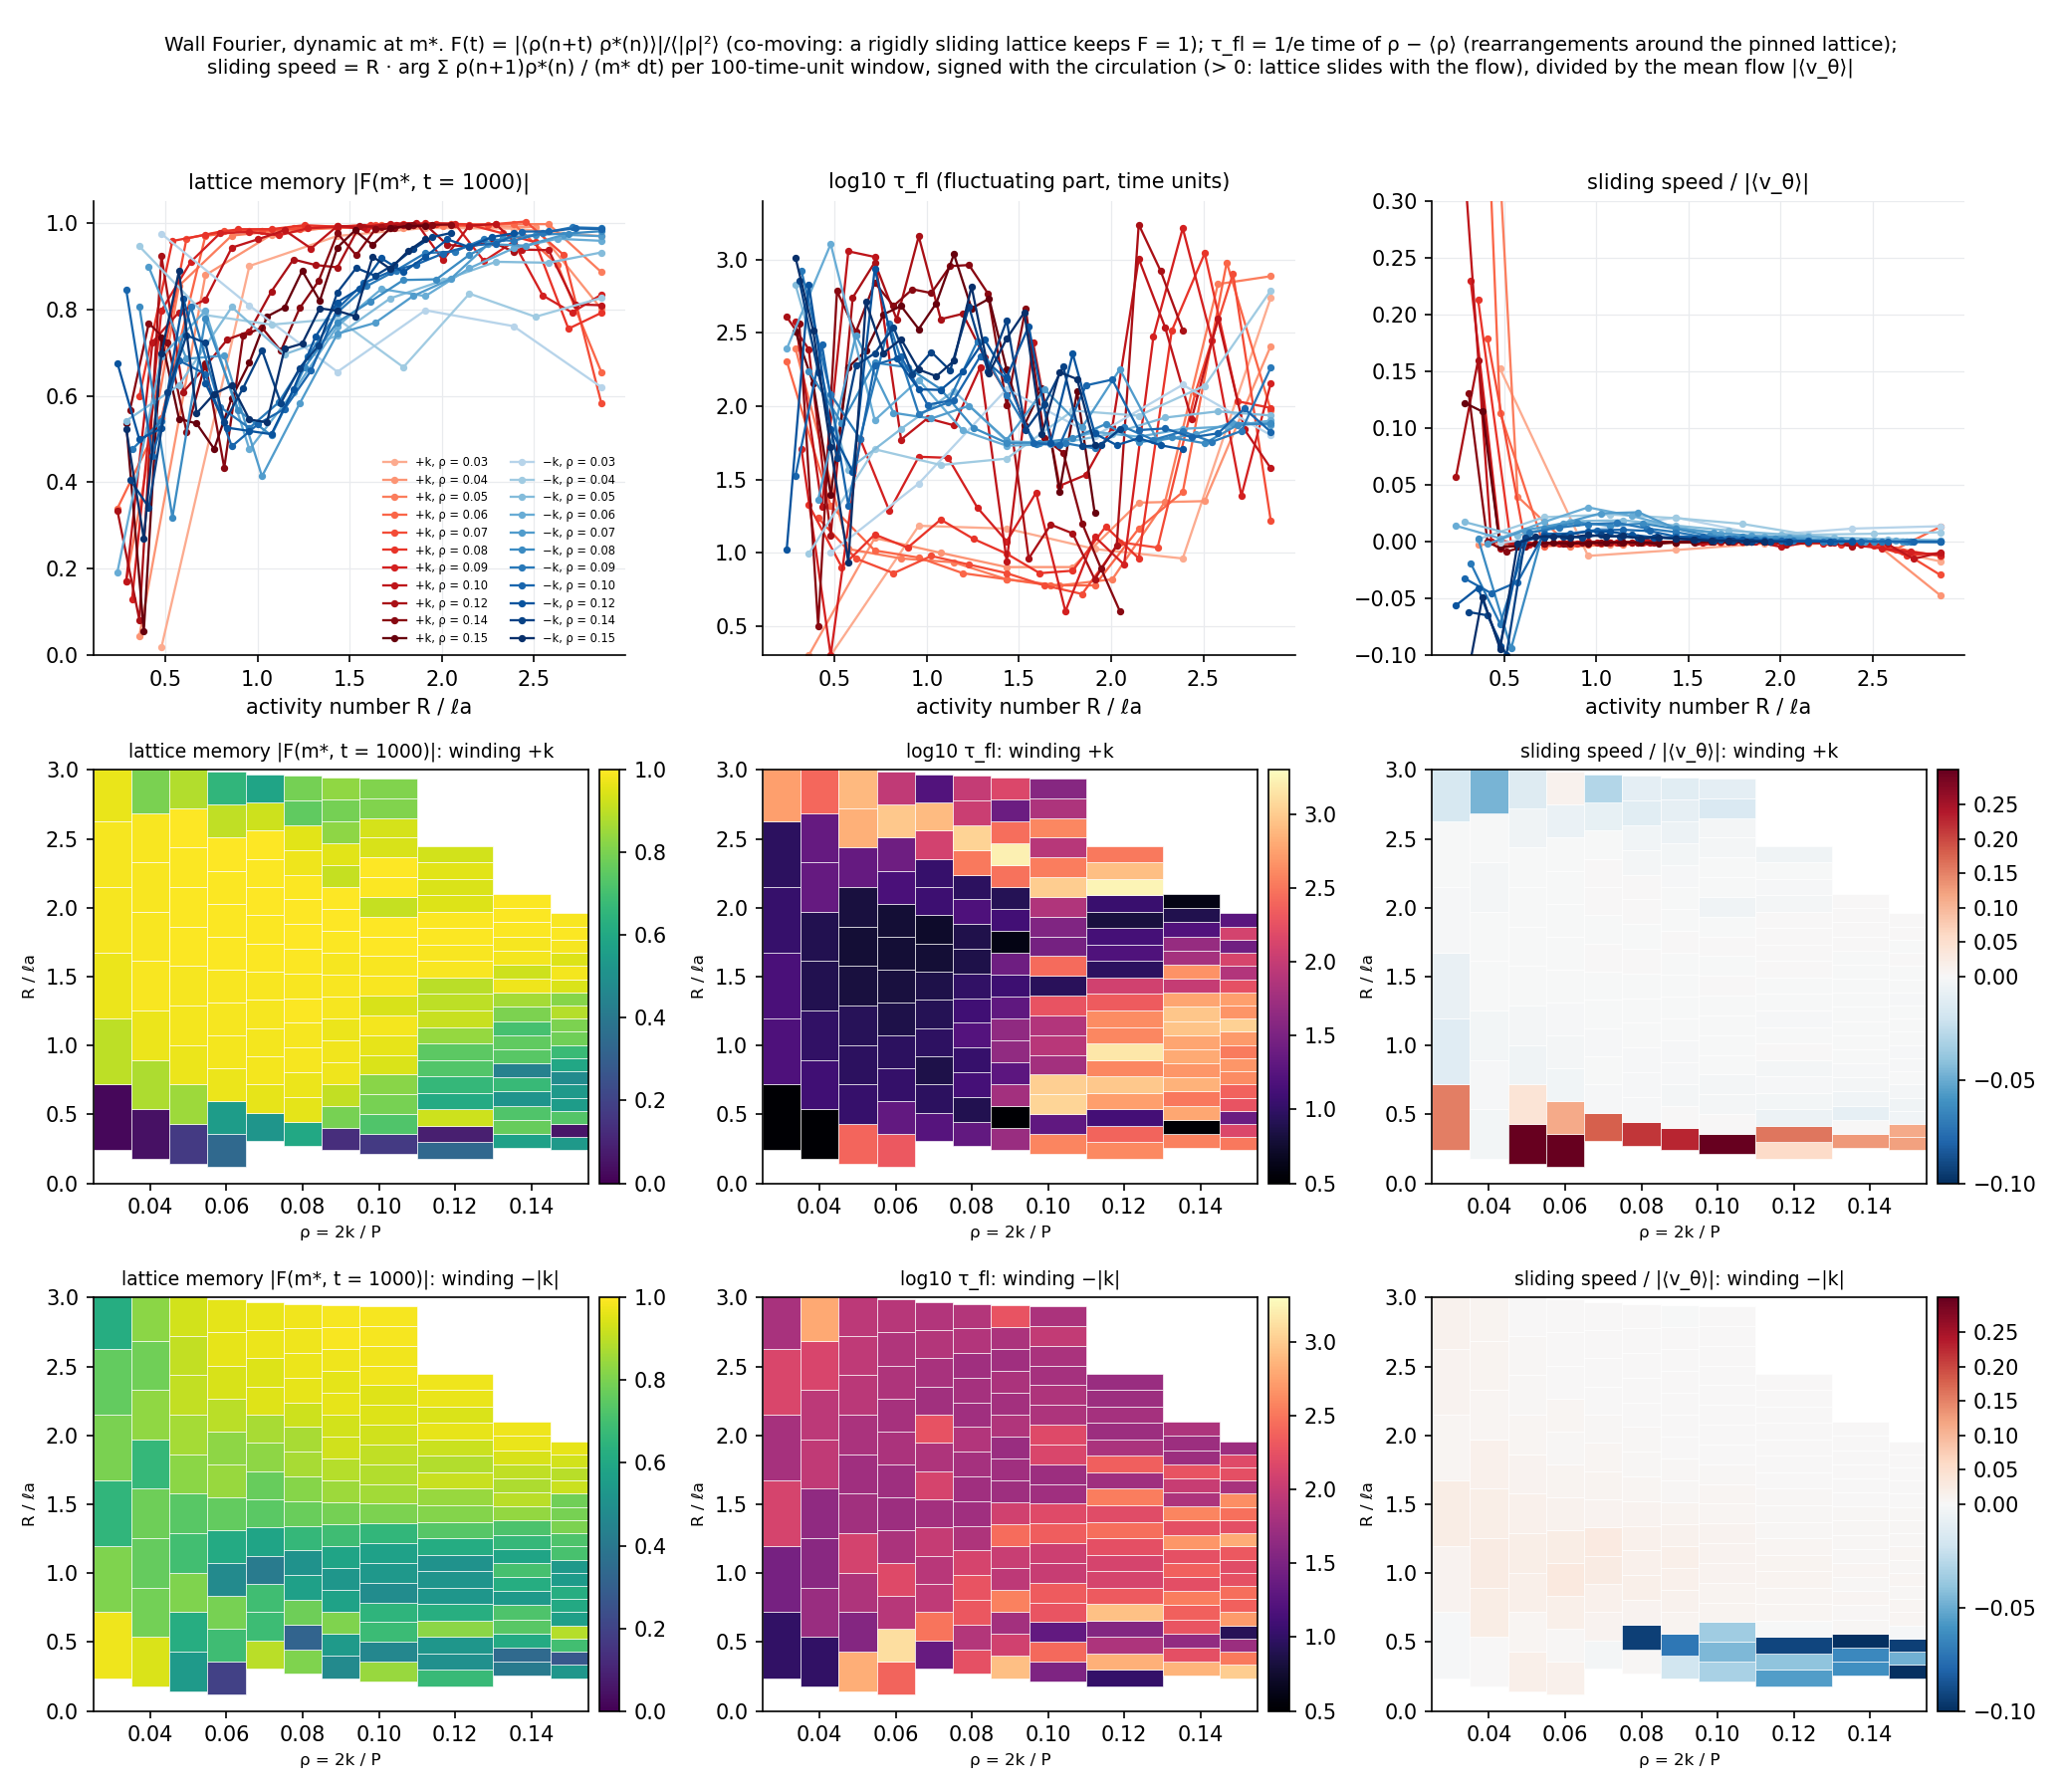
\includegraphics[width=0.85\textwidth]{figs/fourier_dynamic_circles.png}
\caption{Circles, dynamic wall Fourier: lattice memory $F(m^*,1000)$, rearrangement time and lattice sliding speed.}\label{fig:fourier-dyn}
\end{figure}

\subsection{Edge/bulk criteria over the whole sweep}
Six criteria for the bulk charge compared on 930 circle runs (Fig.~\ref{fig:criteria}).
\begin{itemize}
  \item $+k$: all criteria agree on $q_b\approx1$ for $R\approx0.8$--$2\,\la$. The knee of $Q(r)$ is the most robust
        ($\approx1$ from 0.6 to $2.4\,\la$) but undefined at large $R$ and low $\rho$. A fixed-depth cut ($r<11R/12$) fails at
        small and large $R$; density-minimum and mobility give $q_b\to0$ below $0.6$--$0.8\,\la$; slow + tilted overcounts at
        high $\rho$, where the tilt is smaller.
  \item $-|k|$: the knee value rises with $\rho$ and $R$ and reaches 0.9--1 only at $\rho\gtrsim0.10$, $R\gtrsim1.5\,\la$,
        consistent with the vacant wall lattice.
  \item For the paper: the knee as primary criterion, density minimum and mobility as cross-checks, no fixed-depth cut.
\end{itemize}
\begin{figure}[h]\centering
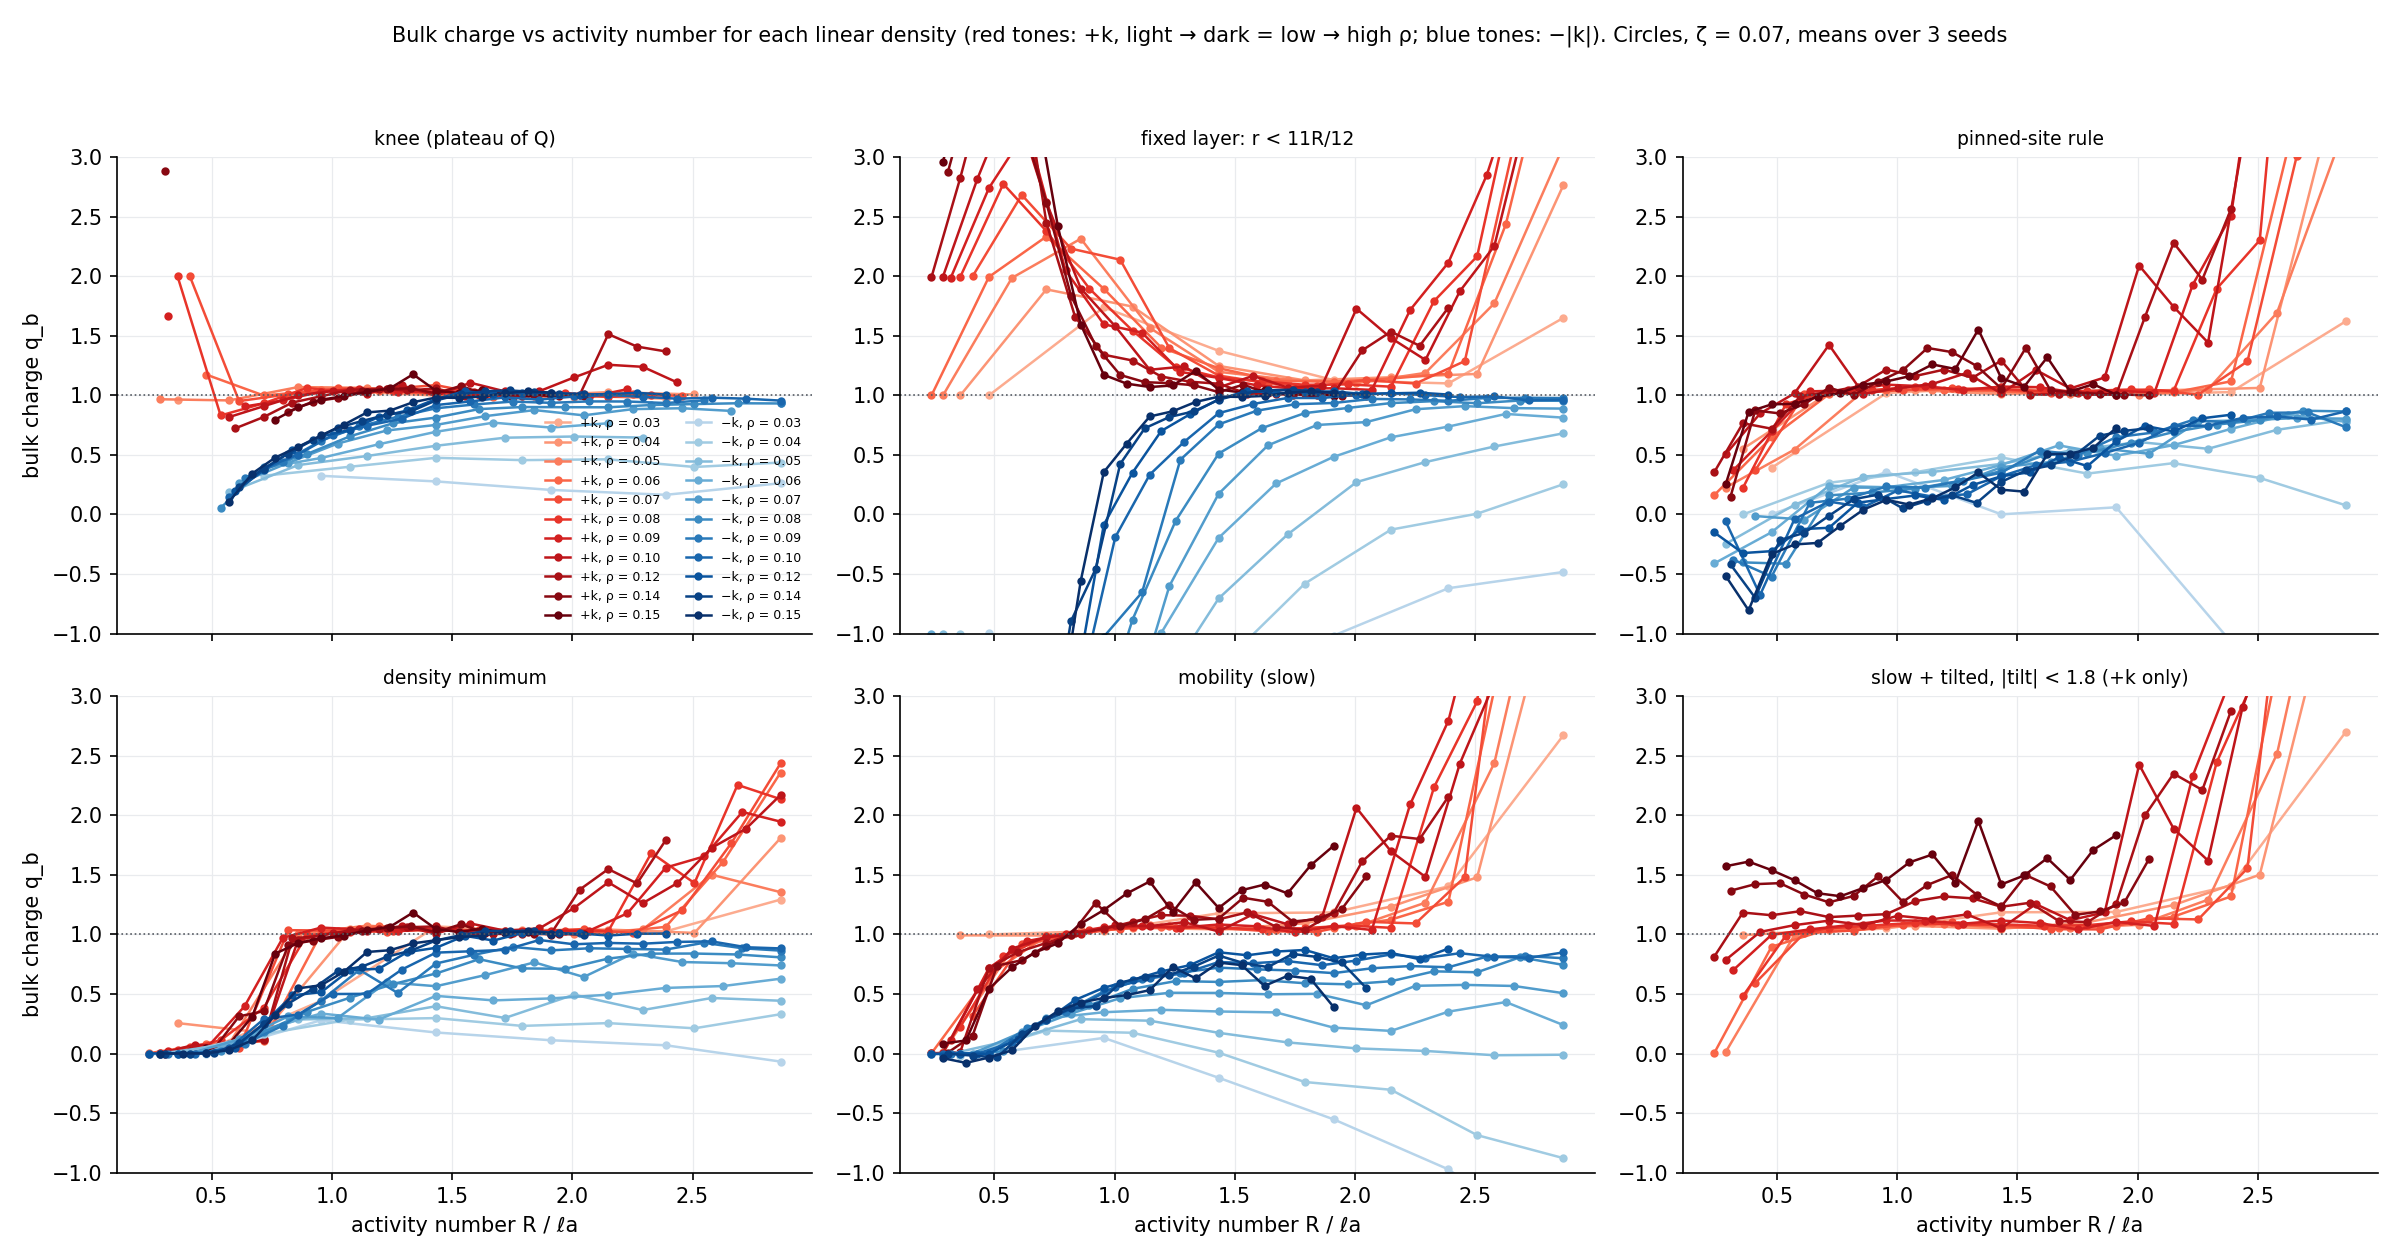
\includegraphics[width=\textwidth]{figs/criteria_bulk_vs_R.png}
\caption{Circles: bulk charge vs $R/\la$ for six edge/bulk criteria (red: $+k$, blue: $-|k|$; one curve per $\rho$).}\label{fig:criteria}
\end{figure}

\subsection{Wall dynamics in ovals and ellipses: upstream drift into vacancies}
The same analysis with positions by arclength along the real wall, for 81 oval and ellipse runs, and with a circle
reference ($k=6$, all $R$) run with the same script (Fig.~\ref{fig:walldyn}). Where the order is weak the phase of the
lattice mode is noise, so we also measure a \emph{per-defect drift}: wall $+\tfrac12$ matched between frames, $ds/dt$
along the wall, signed with the near-wall tangential flow $v_w$ (cells 1--5 from the wall).
\begin{itemize}
  \item No sliding-ordered layer in ovals either: where a lattice exists it is pinned. The near-wall flow turns with the
        bulk vortex (sign agreement 100\% with one strong vortex, 60--90\% in elongated cavities, where $|v_w|$ drops from
        0.2--0.35 to 0.03--0.07).
  \item \textbf{Wall $+\tfrac12$ drift against the wall flow, at a rate set by the vacancies of the wall lattice}, not by
        the loss of pinning: Spearman $\rho_s=-0.82$ between drift$/|v_w|$ and the vacancy fraction $1-N_\mathrm{wall}/(2k-2)$
        over all runs ($-0.93$ among pinned lattices), against $+0.18$ for $f_\mathrm{static}$. Circles ($k=6$): drift
        $\approx0$ for $R=0.7$--$1.7\,\la$, $-2\%$ at 2.15, $-18\%$ at $2.87\,\la$. The H48 $b/a=2.0$ oval is pinned
        ($f=0.84$) but 41\% empty and drifts at $-69\%$; elongated ovals $-10$ to $-80\%$.
  \item Reading: defects hop upstream into empty sites, so vacancies travel downstream. Crowded walls stop the drift:
        in the $k$ scan it vanishes from $k=6$--8 on, and in the pinched oval at $k=12$--20.
  \item Caveats: noisy for tiny circles without a vortex and for single-seed cavities; the drift includes defects entering
        or leaving the wall band.
\end{itemize}
\begin{figure}[h]\centering
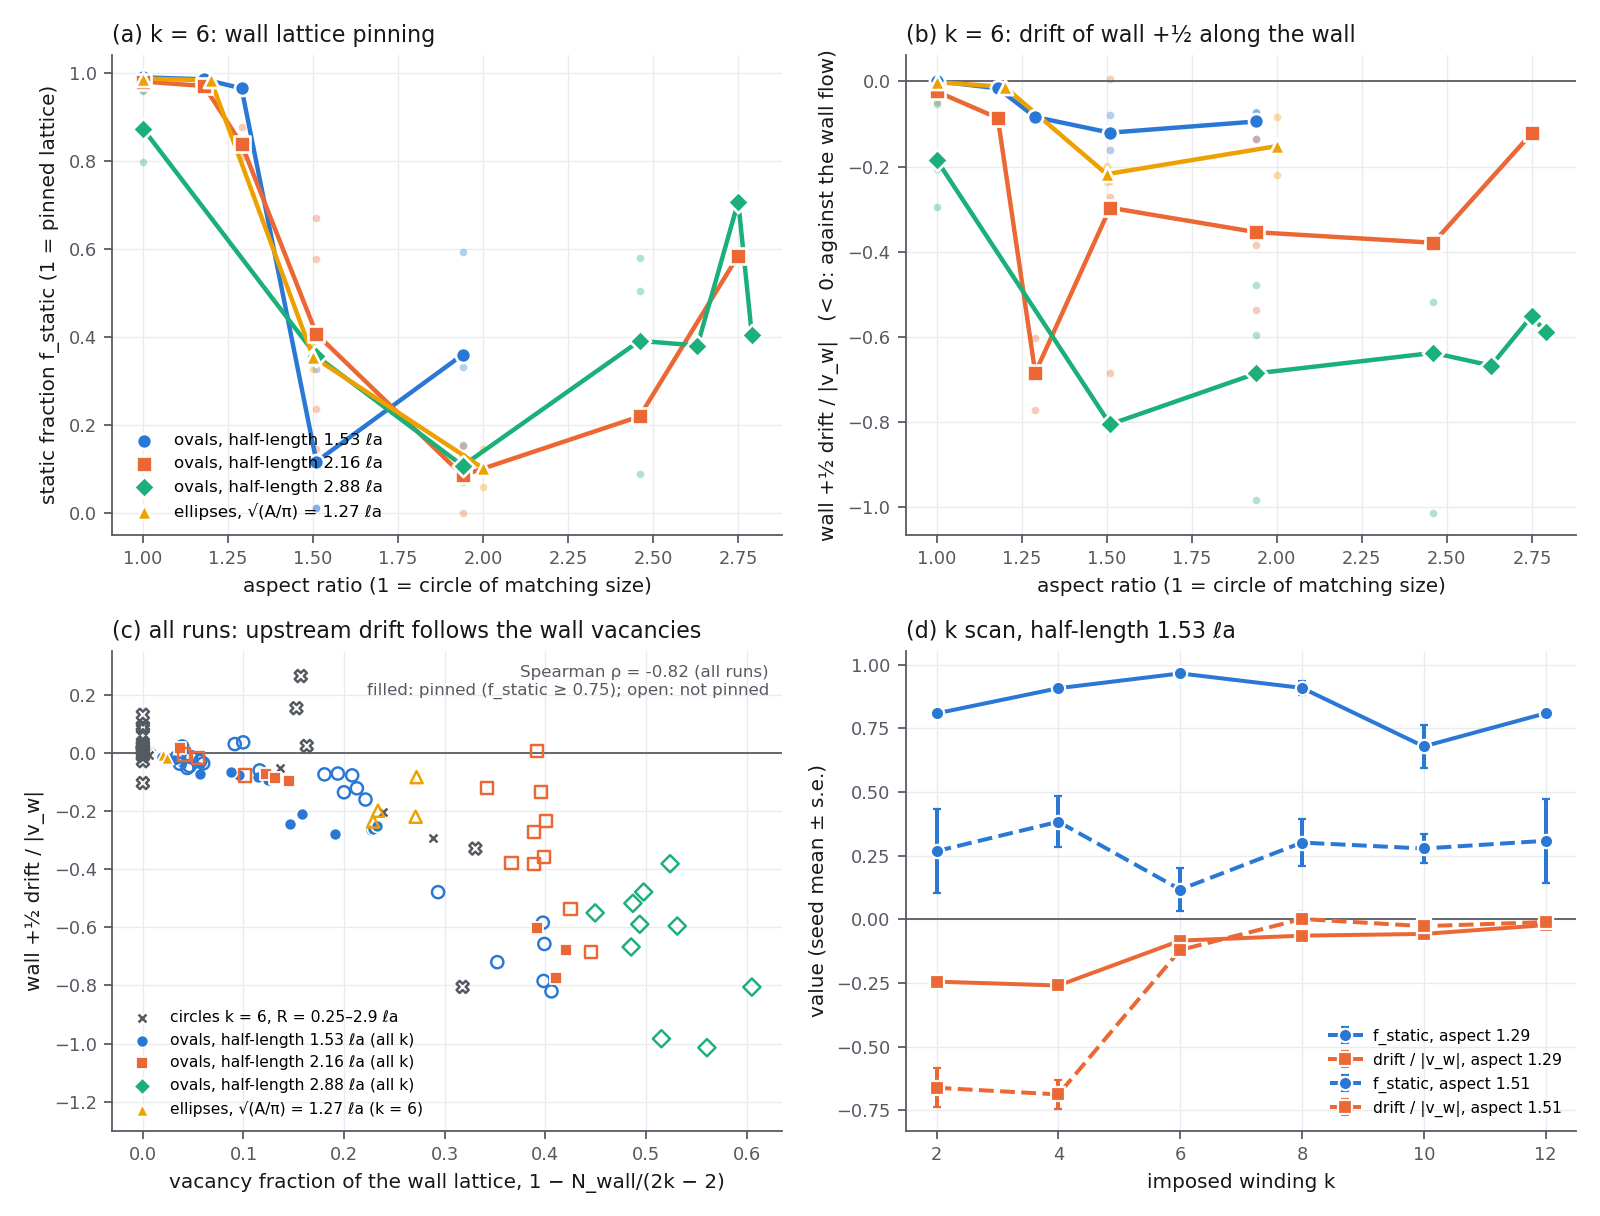
\includegraphics[width=\textwidth]{figs/wall_dynamics.png}
\caption{Ovals and ellipses vs circles. (a) static fraction vs aspect ratio ($k=6$; circles of matching size at aspect 1, in
the colour of the family they match); (b) per-defect drift$/|v_w|$; (c) drift vs vacancy fraction, all runs (filled: pinned,
$f_\mathrm{static}\ge0.75$); (d) $k$ scan at half-length $1.53\,\la$.}\label{fig:walldyn}
\end{figure}
\clearpage


%=====================================================================
\section{Hypotheses: status}
{\small\renewcommand{\arraystretch}{1.25}
\begin{tabularx}{\textwidth}{@{}l>{\raggedright\arraybackslash}p{0.30\textwidth}>{\raggedright\arraybackslash}X@{}}\toprule
& Hypothesis & Status\\\midrule
H1 & Topological or geometric charge split? & \textbf{geometric}: elongation (aspect $\gtrsim1.4$--1.5) destroys the layer in ovals \emph{and} ellipses at matched size and density; a crowded wall (high $k$) pushes back towards topological\\
H2 & Effect disappears at low density & not supported: circles keep the layer at all $\rho\le0.15$ for $R=0.75$--$2\,\la$; size matters (degrades $>2.5\,\la$, $<0.6\,\la$)\\
H3 & Activity only through $\la$ & rejected; $\zeta=0.07$ sweet spot\\
H4 & Bulk $+1$ when the flow circulates & circulation always on in circles; to analyse in the main sweep\\
H5 & Negative winding & bulk stays \emph{positive}, rising to $+1$ only for $|k|\gtrsim13$; activity breaks the mirror symmetry\\
H6 & Wall-layer formation & $2k-2$ pinned sites active vs $2k$ passive; sliding layer at large $R$\\
H7 & Docking at the layer edge & escape rates: circles $\sim0.4\times10^{-3}$, elongated ovals 10--20$\times$ faster; layer empties by undocking\\
H8 & Figure-8: circulation vs topology & two vortices per oval at $b/a\le1.6$; lobes do not decouple at pinch-off; lobe shape alone suffices\\\bottomrule
\end{tabularx}}

%=====================================================================
\section{Computing}
\begin{itemize}
  \item \textbf{Server} (EPYC 9454P, 96 runs at once, 28.7 MPUPS total; clock $\approx2.95$\,GHz all-core with boost on):
        circle sweep complete (batch 1: 568 runs; batches 2+3: 1304 runs incl.\ mirror $-k$; 0 failures; finished 3 Oct).
        \texttt{cassini} binary built and validated; oval sweep drafted, awaiting approval.
  \item \textbf{Office} (7950X): Cassini pilots P1--P3, H3 runs, density checks, analyses; overnight analysis script.
  \item Storage: server SSD only (HDD off-limits); finished runs gzip-compressed.
\end{itemize}

%=====================================================================
\section{Priorities and open items}
\begin{enumerate}
  \item \textbf{H1 evidence (paper 1):} size control done; next: seeds for the half-length-48/64 ovals, the crossover
        in aspect ratio (b/a 2.0--2.5, more shapes and seeds), $k$ dependence (high $k$ restores the layer), same-area comparison;
        then oval sweeps on the server (needs the \texttt{cassini} binary there; build after the current sweeps,
        which also brings the seed fix).
  \item \textbf{Main sweep analysis} (server circles): $Q(c)$ plateau vs $R/\la$ and $\rho$ (H2, H4); mirror runs (H5).
  \item \textbf{Mechanism:} where wall defects go, exchange rates, lobe vortices; pinch-off reference (a lobe-sized
        cavity at winding $\approx k/2$).
  \item Ellipses on the office machine (convex cavities; second family).
  \item Maintenance: server rebuild; checkpoint-restart crash; send the upstream report; merge \texttt{cassini}.
  \item Communication: update the collaborator brief (v5) with the H1 figure.
\end{enumerate}
\textbf{To discuss with Tyler:} ovals in paper 1; how much of the density-stratification analysis goes into the SI;
whether a low-Mach control is worth the recalibration.

\appendix
\section{Where things are}
\begin{tabularx}{\textwidth}{lX}\toprule
Notes & \texttt{RESEARCH.md} (status first, dated results log), \texttt{TODO.md}\\
Circles & \texttt{runs/cavity/} (R-scan, H3pilot, H3high, density\_check, server\_k06, analysis\_spatial/)\\
Ovals & \texttt{runs/cassini/} (P1, P2, P3, movies/, figures)\\
Calibration & \texttt{runs/activeLength/} (L100, L200, compressibility)\\
Code & \texttt{mpcd/} (production), \texttt{niamh-overcharged/} (git: main, cassini)\\
Reports & \texttt{reports/} (brief, bug report, Cassini patch plan, this report)\\\bottomrule
\end{tabularx}
\end{document}
